% version 1.01	Auteur Julie Pain, Pierre Porche

\documentclass[asi]{picInsa}
\DeclareGraphicsRule{*}{pdf}{*}{}
\usepackage{pdfpages}


\usepackage{vocabulaireUnipik}

\setcounter{secnumdepth}{4}
\setcounter{tocdepth}{4}
\newcommand{\ligneMaj}[3] {
	\rowcolor[gray]{0.55} \textbf{\textit{#1}} & #2  &  #3\\
	\hline
}
\newcommand{\ligneSup}[3] {
	\rowcolor[gray]{0.65} |\textunderscore \textbf{\textit{#1}} & #2  &  #3\\
	\hline
}
\newcommand{\ligneMed}[3] {
	\rowcolor[gray]{0.75} \hspace{0.25cm} |\textunderscore #1  & #2 & #3 \\
	\hline
}
\newcommand{\ligneSub}[3] {
	\rowcolor[gray]{0.85}  \hspace{0.5cm} |\textunderscore #1 & #2 & #3\\
	\hline
}
\newcommand{\ligneSubSub}[3] {
	\rowcolor[gray]{0.95}  \hspace{0.75cm} |\textunderscore #1 & #2 & #3\\
	\hline
}
\newcommand{\ligneTache}[3] {
	\hspace{1.00cm} |\textunderscore #1 & #2 & #3\\
	\hline
}
\title{\PQ{}}
\author{\Pierre}


\titreGeneral{\PQ}
\sousTitreGeneral{\nomEquipe}
\titreAcronyme{\PQCourt}
\version{v1.01}
\titreDetaille{\PQCourt\_Q\_\nomEquipe\_\versionPrive}
\referenceVersion{\PQCourt\_Q\_\nomEquipe\_\versionPrive}
\auteurs{\Kafui{} \& \Melissa{} \& \Sergi{} \& \Michel{} \& \Florian{} \&  \Julie{} \& \Pierre{}}
\destinataires{\nomApprobateur{}, \nomTuteurQualite, \nomEquipe}
\resume{Le présent document contient la présentation du \PQ{} \nomEquipe.}
\motsCles{\PQCourt{}, référentiel, nommage}
\natureDerniereModification{Correction}
\modeDiffusionControle{}

\begin{document}

\couverture{}

 \informationsGenerales{}
% version 1.00, date 29/02/16, auteur Michel Cressant
\begin{pagesService}
	\begin{historique}
		% nouvelles versions à rajouter AU-DESSUS en recopiant les lignes suivantes et en les modifiant :
		\unHistorique{1.00}{02/02/2016}{\Michel}{Création}{Toutes}

	\end{historique}

%        \begin{suiviDiffusions}
%
%            % On place ici les diffusions
%        	\unSuivi{1.00}{}{\nomEquipe{}}
%          
%          
%        \end{suiviDiffusions}

%%Signataires
        \begin{signatures}
	   \uneSignature{Vérificateur}{\RRS}{\Matthieu{}}{17/03/2016}{PGPic}
       \uneSignature{Validateur}{\CP{}}{\Sergi}{}{PGPic}
        \end{signatures}
	
	

	
	
\end{pagesService}


\tableofcontents

\setcounter{chapter}{0}
 
\chapter{Fiche projet}
\label{fiche_projet}
		Le présent document présente le \PQ{} du PIC UNICEF qui sera désigné sous le nom de "\nomEquipe" pour tous les documents liés à ce PIC. L'objectif de ce \PQ{} est de décrire l'ensemble des modes opératoires, des ressources et de la séquence des activités liées à ce projet. Il aide à démontrer que \nomEquipe{} est capable de fournir un produit conforme aux exigences du client et à la norme \ISO . \\
		
		Des contrôles réguliers seront effectués afin de vérifier la bonne application de la démarche décrite dans ce \PQ .\\
		
		La direction ainsi que l'ensemble des membres de l'équipe \nomEquipe{} s'engagent à respecter les dispositions décrites dans ce \PQ .\\ 
		

		
	\begin{description}
		\item[Sujet du PIC~:] "L'objectif est de permettre une gestion informatisée par les divers responsables des actions et des comités départementaux des actions à venir, en cours et passées" sur les trois programmes suivants : plaidoyers, les poupées Frimousse et les actions liées aux Jeunes Ambassadeurs. \\	
		\item[Intitulé du PIC~:] PIC \nomPIC \\	
		\item[Nom de l'équipe PIC~:] \nomEquipe \\
	\end{description}


\noindent\hfil\rule{\textwidth}{.4pt}\hfil


		
\section*{Cahier des charges}
		\subsection*{Besoin à satisfaire~:} 
		Permettre une gestion informatisée des interventions externes de l'UNICEF 76 dont : plaidoyers, poupées Frimousse, actions liées aux Jeunes Ambassadeurs.
		\\	cf. \DSE . 		
		\subsection*{Élements à livrer~:}
		Un outil de gestion des interventions.
		\\	cf. \DSE
			
					


	\vspace{1cm}
	\noindent\hfil\rule{\textwidth}{.4pt}\hfil
	\vspace{1cm}	
	
	
\section*{Informations sur le client}
	\begin{description}
		\item[Nom de l'organisme~:] UNICEF Haute Normandie \\
		\item[Nom de son représentant~:] Véronique BARBIER \\
		\item[Adresse de l'organisme~:] 26 rue Saint Nicolas, 76000 Rouen \\
		\item[Téléphone~:] 02 35 88 98 88 \\
		\item[E-mail~:] president.unicef76@unicef.fr \\
	\end{description}
	
	
	\vspace{1cm}
	\noindent\hfil\rule{\textwidth}{.4pt}\hfil
	\vspace{1cm}	
	
\section*{Informations complémentaires}
	
	\begin{description}
	
		\item[Nom du tuteur pédagogique~:] \nomTuteurPedago \\
		\item[Nom du tuteur qualité~:] \nomTuteurQualite \\
		\item[Lieu de réalisation du projet~:] \adresseSalle \\
		\item[Nombre d'élèves ingénieur de l'équipe 
PIC~:] 9 \\
		\item[Fonds alloués au projet par le département \ASICourt{}~:] 700 \euro{}
	\end{description}	
	
	\noindent\hfil\rule{\textwidth}{.4pt}\hfil	
	
	\section*{Aspect contractuel}
	
	
	\begin{tabular}[h]{|p{0.3\textwidth}|p{0.6\textwidth}|}
	\hline
	
	\cellcolor{gray!40}Membre équipe PIC & \cellcolor{gray!40}Rôle(s) \\\hline
	\Sergi & \CP \\\hline
	\Pierre & \CPA , \RQ \\\hline
	\Michel & \D , \RD \\\hline 
	\Kafui  & \D , \RQA \\\hline
	\Matthieu & \D , \RRS \\\hline
	\Mathieu & \D , \RGC \\\hline
	\Melissa  & \D \\\hline
	\Julie & \D \\\hline
	\Florian & \D \\\hline
	
\end{tabular}
	
	\vspace{1cm}
	\noindent\hfil\rule{\textwidth}{.4pt}\hfil
	\vspace{1cm}	
	
	\section*{Propriété intellectuelle}
		\begin{itemize}
			\item Copropriété $\square$
			\item Propriété INSA $\square$
			\item Propriété entreprise $\boxtimes$
		\end{itemize}
	
		


\chapter{Engagements}
\label{egagements}
% version 1.00, date 20/01/16, auteur Michel Cressant
Tous les signataires ont pris connaissance du présent Plan Qualité et s'engagent à respecter ses exigences. \\
	
	\vspace{1cm}

\begin{tabular}[h]{|p{0.25\textwidth}|p{0.40\textwidth}|p{0.12\textwidth}|p{0.12\textwidth}|}
	\hline
	
	\cellcolor{gray!40}Membre équipe PIC & \cellcolor{gray!40}Rôle(s) dans le projet & \cellcolor{gray!40}Date & \cellcolor{gray!40}Signature \\\hline
	\Pierre 	& \CP 			& & \\\hline
	\Francois 	& \CPA \newline \D 	& & \\\hline 
	\Kafui  	& \RQ 			& & \\\hline
	\Matthieu 	& \D \newline \RRS 	& & \\\hline
	\Florian 	& \D \newline \RS 	& & \\\hline
	\Melissa  	& \D \newline \RGC 	& & \\\hline
	\Julie 		& \D \newline \RD 	& & \\\hline
	\Juliana 	& \D 			& & \\\hline
\end{tabular}




\chapter{Décomposition en fonction des membres (WBS)}
\label{decomposition_membre_WBS}
\section{Décomposition en activités des processus du PIC}

Le Système de Management de la Qualité défini par le PIC \nomPIC{} se décompose en trois processus~:
\begin{itemize}
 \item Manager la qualité : assurer, suivre et améliorer la qualité du \PICCourt ; 
 \item Conduire le projet ;
 \item Réaliser les produits. \\
\end{itemize}

Un pilote (membre du \PICCourt) est attribué à chaque processus. Sa mission sera de s'assurer du bon fonctionnement du processus et de gérer les risques liés à ce dernier.

Pour diviser le projet en processus, nous avons utilisé un \WBS{} (\WBSCourt). Le \WBSCourt{} est visible sur la figure \ref{WBS1}.

\begin{figure}[H]
\centering
 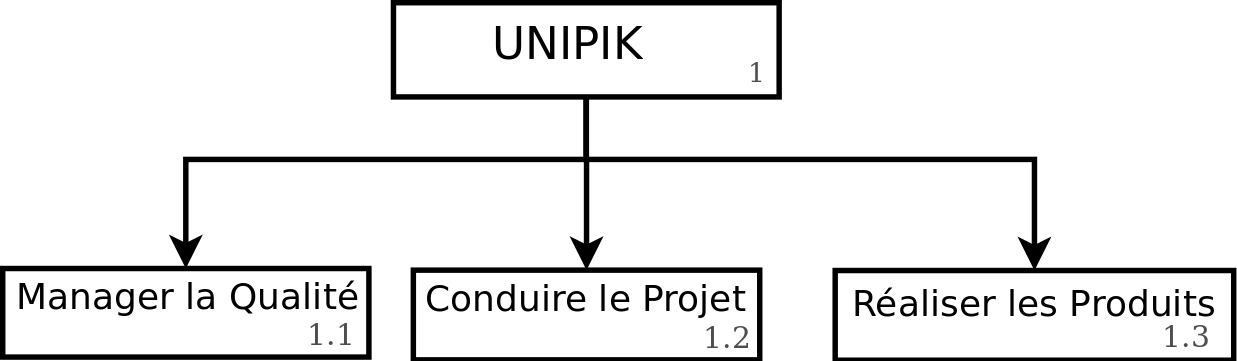
\includegraphics[width=14cm]{images/organigramme_processus_pic.png}
 \caption{Processus du PIC~: projet \nomEquipe{}}
 \label{WBS1}
\end{figure}

 Dans le cas où il y a des évolutions, les modifications seront présentées dans la prochaine mise à jour.
\newpage
 
\section{Processus : Manager la Qualité}
\label{ProcessusQualite}
Ce processus se décompose en trois parties:
\begin{itemize}
\item La mise en place de la Qualité au sein du \PICCourt{} (rédaction du \PQ{} et organisation de l'équipe \PICCourt) ; 
\item Le suivi de la Qualité tout au long du projet ; 
\item L'amélioration de la Qualité tout au long du \PICCourt{} (définition d'objectifs et d'axes d'amélioration et mise à jour des documents). 
\end{itemize}
\subsection{\WBSCourt{}}
Le \SMQ{} au moment de la diffusion de ce document est présenté par une \WBSCourt, disponible en figure 3.2.
Le pilote de ce processus sera \Pierre{} en tant que \RQ{}.
\newpage
\begin{figure}[H]
\centering
 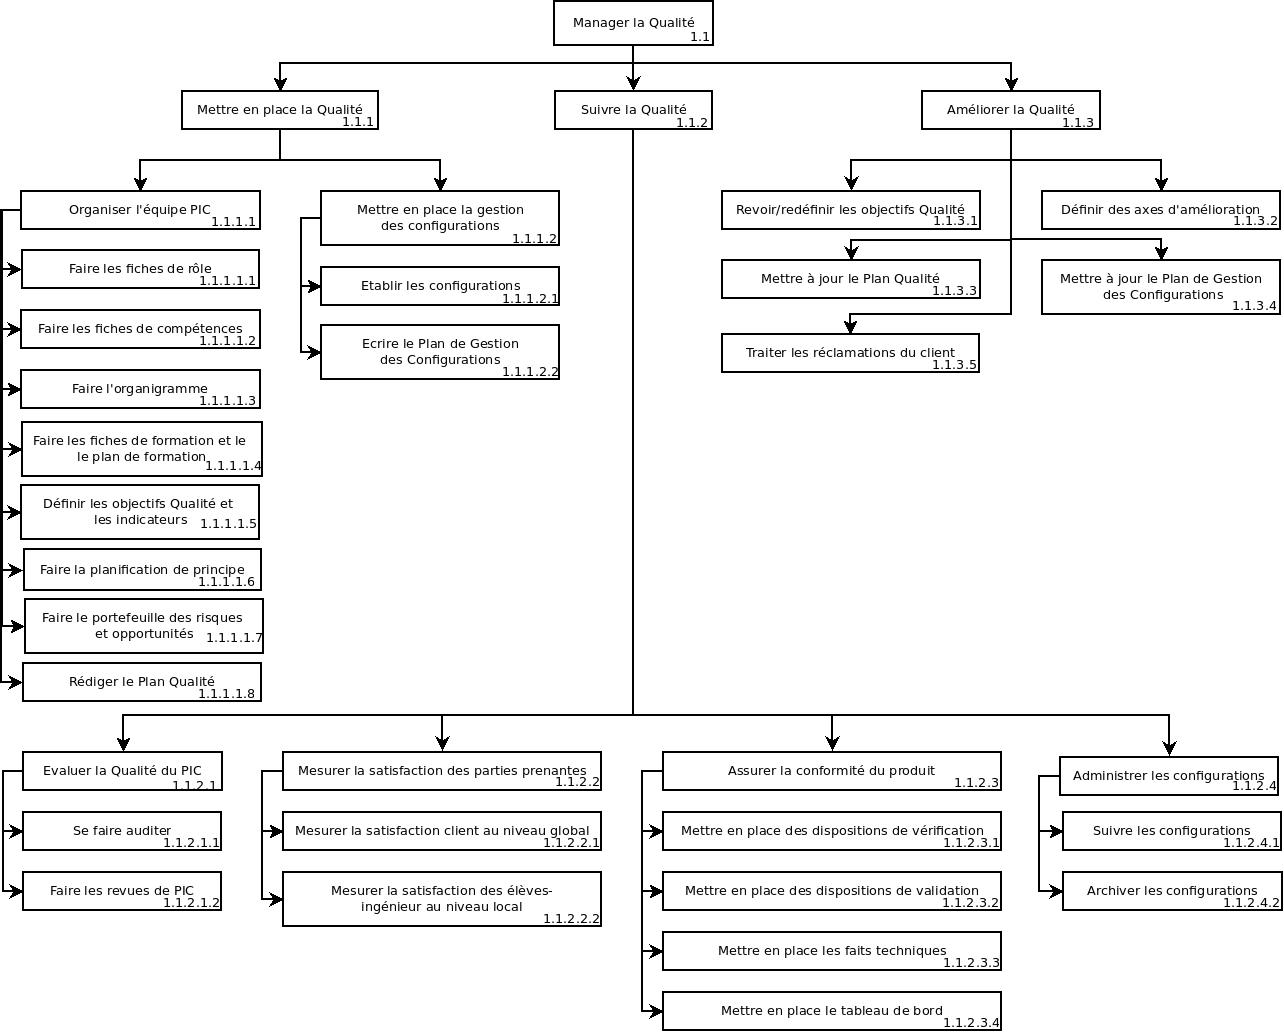
\includegraphics[width=23cm,angle=90]{images/manager_qualite.png}
 \caption{\WBSCourt{}~: Manager la Qualité}
 \label{WBS2}
\end{figure}

\newpage
\begin{landscape}
\subsection{Références aux procédures}

\begin{longtable}{|p{3cm}|p{14.5cm}|p{5cm}|}
	% En-tête du tableau
	\hline
	\rowcolor[gray]{0.65}\textbf{N° WBS} & \textbf{Intitulé du processus / de l'activité / de la tâche} & \textbf{Procédure en référence}\\
	\hline
	\endhead % (répétée, sinon \endfirsthead)

	% Corps du tableau


        \ligneMaj{1.1}{Manager la qualité}{Chapitre 4 - \DGQDEUXCourt{}}

        \ligneSup{1.1.1}{Mettre en place la qualité}{Partie 4.2 - \DGQDEUXCourt{}}
        \ligneMed{1.1.1.1}{Organiser l'équipe PIC}{Partie \ref{Organisation} - \PQCourt{}}
        \ligneSub{1.1.1.1.1}{Faire les fiches de rôle}{Partie \ref{RolesEtCompetences} - \PQCourt{}}
        \ligneSub{1.1.1.1.2}{Faire les fiches de compétences}{Partie \ref{RolesEtCompetences} - \PQCourt{}}
        \ligneSub{1.1.1.1.3}{Faire l'organigramme}{Partie  \ref{Organisation} - \PQCourt{}}
        \ligneSub{1.1.1.1.4}{Faire les fiches de formation et le plan de formation}{Partie \ref{formation} - \PQCourt{}}
        \ligneSub{1.1.1.1.5}{Définir les objectifs Qualité et les indicateurs}{Partie \ref{qualite} - \PQCourt{}}
        \ligneSub{1.1.1.1.6}{Faire la planification de principe}{Partie  \ref{planning_de_principe} - \PQCourt{}}
        \ligneSub{1.1.1.1.7}{Faire le portefeuille des risques et opportunités}{Partie  \ref{gestion_risques_opportunitees} - \PQCourt{}}
        \ligneSub{1.1.1.1.8}{Rédiger le Plan Qualité}{Partie 4.2.2 - \DGQDEUXCourt{}}
        \ligneMed{1.1.1.2}{Mettre en place la gestion des configurations}{Partie 7.2 - \DGQDEUXCourt{}}

        \ligneSup{1.1.2}{Suivre la Qualité}{Partie 4.3 - \DGQDEUXCourt{}}
        \ligneMed{1.1.2.1}{Évaluer la Qualité du PIC}{}
        \ligneSub{1.1.2.1.1}{Se faire auditer}{Partie 4.3.4 - \DGQDEUXCourt{}}
        \ligneSub{1.1.2.1.2}{Faire les revues de PIC}{Partie 4.3.3 \DGQDEUXCourt{}}
        \ligneMed{1.1.2.2}{Mesurer la satisfaction des parties prenantes}{Partie 4.3.1 \DGQDEUXCourt{}}
        \ligneSub{1.1.2.2.1}{Mesurer la satisfaction client au niveau global}{Partie 3.1.1 - \DGQTROISCourt{}}
        \ligneSub{1.1.2.2.2}{Mesurer la satisfaction des élèves-ingénieur au niveau local}{Partie 3.1 - \DGQTROISCourt{}}
        \ligneMed{1.1.2.3}{Assurer la conformité du produit}{}
        \ligneSub{1.1.2.3.1}{Mettre en place des dispositions de vérification}{Partie 4.3.2 - \DGQDEUXCourt{}}
        \ligneSub{1.1.2.3.2}{Mettre en place des dispositions de validation}{Partie 4.3.2 - \DGQDEUXCourt{}}
        \ligneSub{1.1.2.3.3}{Mettre en place les faits techniques}{Partie 4.3.5 - \DGQDEUXCourt{}}
        \ligneSub{1.1.2.3.4}{Mettre en place le tableau de bord}{Partie 4.3.6 - \DGQDEUXCourt{}}
        \ligneMed{1.1.2.4}{Administrer les configurations}{Partie 7.3 - \DGQDEUXCourt{}}
        \ligneSub{1.1.2.4.1}{Suivre les configurations}{Partie 4 - \pgcCourt{}}
        \ligneSub{1.1.2.4.2}{Archiver les configurations}{Partie 7 - \pgcCourt{}}

        \ligneSup{1.1.3}{Améliorer la Qualité}{Partie 4.4 - \DGQDEUXCourt{}}
        \ligneMed{1.1.3.1}{Revoir/redéfinir les objectifs Qualité}{Partie 5.2.1 - \DGQTROISCourt{}}
        \ligneMed{1.1.3.2}{Définir des axes d’amélioration}{Partie 4.4.2 - \DGQDEUXCourt{}}
        \ligneMed{1.1.3.3}{Mettre à jour le Plan Qualité}{Partie 4.4.3 - \DGQDEUXCourt{}}
        \ligneMed{1.1.3.4}{Mettre à jour le Plan de Gestion des Configurations}{Partie 4.4.3 - \DGQDEUXCourt{}}
\end{longtable}
\end{landscape}

\newpage



\section{Processus : Conduire le PIC}
\subsection{\WBSCourt{}}
\label{ProcessusConduirePic}
Une \WBS{} qui explique la conduite du projet au moment de la diffusion de ce document est disponible en figure 3.3.
Le pilote de ce processus sera \Sergi{} en tant que \CP{}.
\newpage
\begin{figure}[H]
\centering
 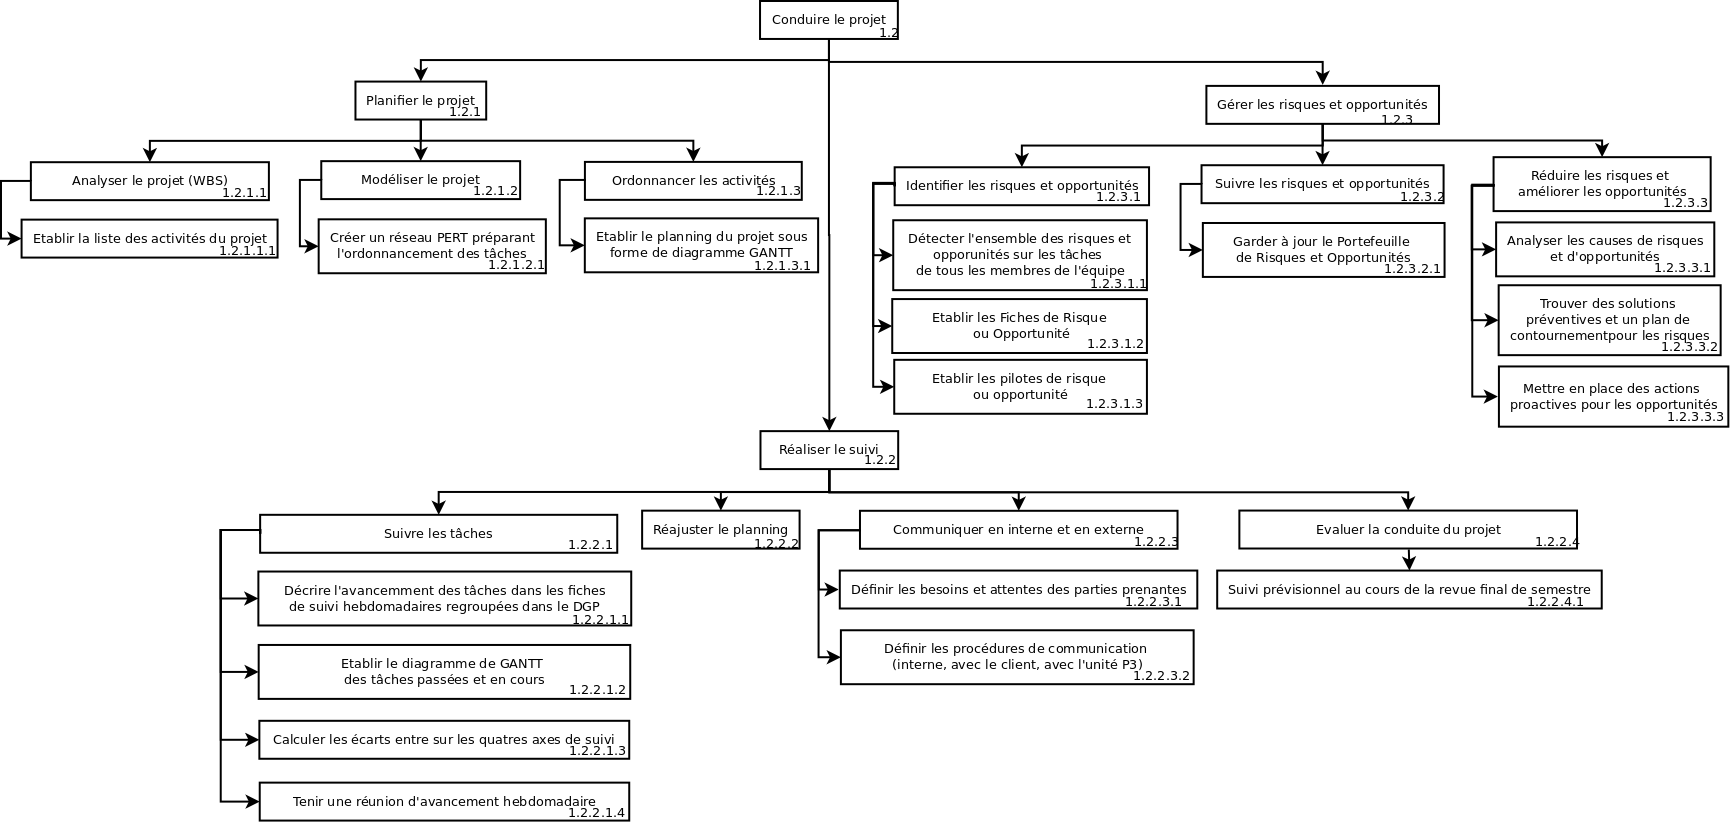
\includegraphics[width=24cm,angle=90]{images/conduire_le_projet.png}
 \caption{\WBSCourt{}~: Conduire le PIC}
 \label{WBS3}
\end{figure}


\newpage
\begin{landscape}
\subsection{Références aux procédures}
		\small
		\begin{longtable}{|p{3.0cm}|p{14.5cm}|p{5cm}|}
			% En-tête du tableau
			\hline
			\rowcolor[gray]{0.65}\textbf{N° WBS} & \textbf{Intitulé du processus / de l'activité / de la tâche} & \textbf{Procédure en référence}\\
			\hline
			\endhead % (répétée, sinon \endfirsthead)

			\ligneMaj{1.2}{Conduire le projet}{Chapitre 5 - \DGQDEUXCourt{}}

			\ligneSup{1.2.1}{Planifier le projet}{Partie 5.2 - \DGQDEUXCourt{}}
			\ligneMed{1.2.1.1}{Analyser le projet (WBS)}{Partie 5.2.1 - \DGQDEUXCourt{}}
			\ligneSub{1.2.1.1.1}{Établir la liste des activités du projet}{}
			\ligneMed{1.2.1.2}{Modéliser le projet}{Partie 5.2.2 - \DGQDEUXCourt{}}
			\ligneSub{1.2.1.2.1}{Créer un réseau PERT préparant l'ordonnancement des tâches}{}
			\ligneMed{1.2.1.3}{Ordonnancer les activités}{Partie 5.2.3 - \DGQDEUXCourt{}}
			\ligneSub{1.2.1.3.1}{Établir le planning du projet sous forme de diagramme GANTT}{}


			\ligneSup{1.2.2}{Réaliser le suivi}{Partie 5.3 - \DGQDEUXCourt{}}
			\ligneMed{1.2.2.1}{Suivre les tâches}{Partie 5.3.1 - \DGQDEUXCourt{}}
			\ligneSub{1.2.2.1.1}{Décrire l’avancement de ses tâches dans les fiches de suivi hebdomadaires regroupées dans le DGP}{}
			\ligneSub{1.2.2.1.2}{Établir le diagramme de GANTT des tâches passées et en cours}{}
			\ligneSub{1.2.2.1.3}{Calculer les écarts entre sur les quatre axes de suivi}{}
			\ligneSub{1.2.2.1.4}{Tenir une réunion d'avancement hebdomadaire}{}
			\ligneMed{1.2.2.2}{Réajuster le planning}{Partie 5.3.2 - \DGQDEUXCourt{}}
			\ligneMed{1.2.2.3}{Communiquer en interne et en externe}{Partie 5.3.3 - \DGQDEUXCourt{}}
			\ligneSub{1.2.2.3.1}{Définir les besoins et attentes des parties prenantes}{}
			\ligneSub{1.2.2.3.2}{Définir les procédures de communication (interne, avec le client, avec l'unité P3)}{}
			\ligneMed{1.2.2.4}{Évaluer la conduite du projet}{Partie 5.3.4 - \DGQDEUXCourt{}}
			\ligneSub{1.2.2.4.1}{Suivi prévisionnel au cours de la revue final de semestre}{}

			\ligneSup{1.2.3}{Gérer les risques et opportunités}{Partie 5.4 - \DGQDEUXCourt{}}
			\ligneMed{1.2.3.1}{Identifier les risques et opportunités }{Partie 5.4.1 - \DGQDEUXCourt{}}
			\ligneSub{1.2.3.1.1}{Détecter l'ensemble des risques sur les tâches de tous les membres de l'équipe}{}
			\ligneSub{1.2.3.1.2}{Établir les Fiches de Risque ou Opportunité}{}
			\ligneSub{1.2.3.1.3}{Établir les pilotes de risque ou opportunité}{}
			\ligneMed{1.2.3.2}{Suivre les risques et opportunités}{Partie 5.4.2 - \DGQDEUXCourt{}}
			\ligneSub{1.2.3.2.1}{Garder à jour le Portefeuille de Risques et Opportunités}{}
			\ligneMed{1.2.3.3}{Réduire les risques et améliorer les opportunités}{Partie 5.4.3 - \DGQDEUXCourt{}}
			\ligneSub{1.2.3.3.1}{Analyser les causes de risques et d'opportunités}{}
			\ligneSub{1.2.3.3.2}{Trouver des solutions préventives et un plan de contournement pour les risques}{}
			\ligneSub{1.2.3.3.3}{Mettre en place des actions proactives pour les opportunités}{}
		\end{longtable}
	\end{landscape}

	\normalsize
	\newpage

\section{Processus : Réaliser les produits}
\subsection{\WBSCourt{}}
\label{ProcessusRealiserProduit}
Une \WBS{} représentant la réalisation des produits au moment de la diffusion du présent document est disponible en figure \ref{WBS5}.
Le pilote de ce processus sera \Michel{} en tant que \RD{}.
\newpage
\begin{figure}[H]
\centering
 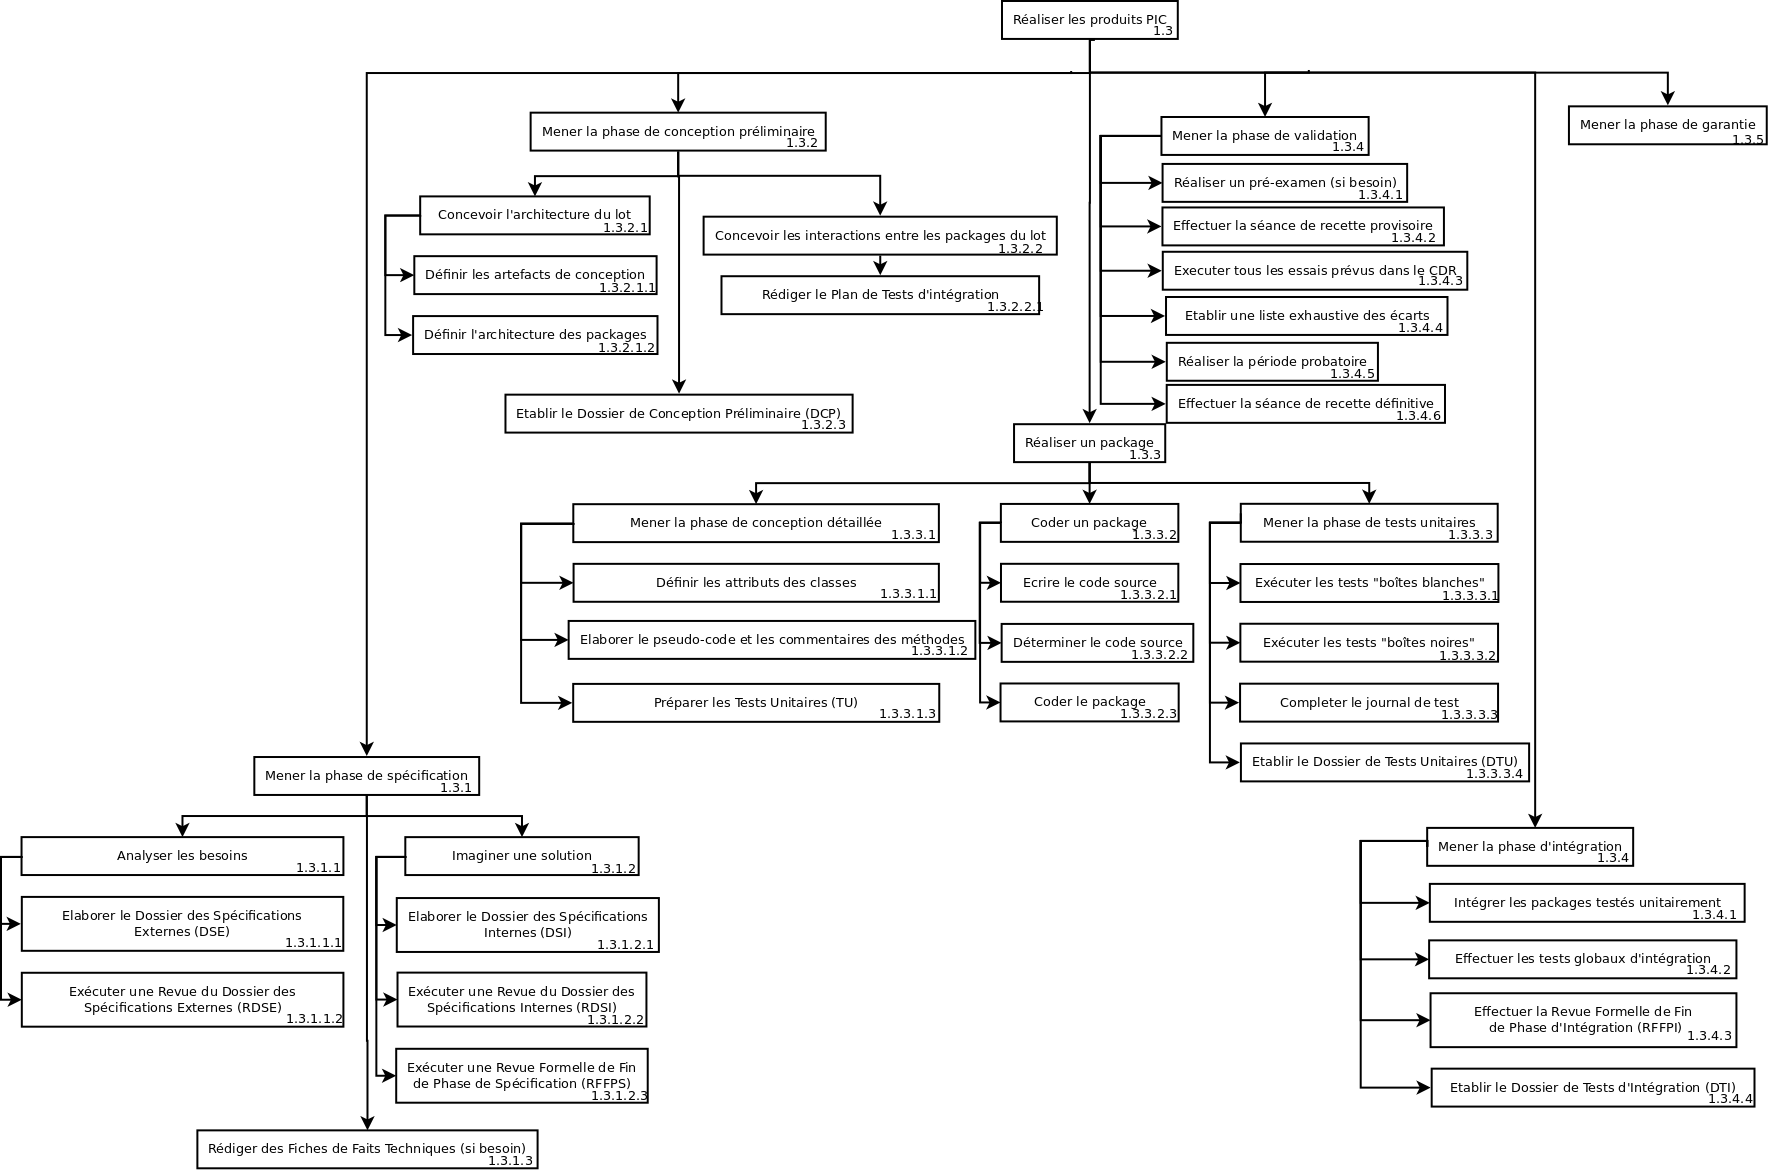
\includegraphics[width=24cm,angle=90]{images/realiser_produits.png}
 \caption{\WBSCourt{}~: Réaliser les produits}
\label{WBS5}
\end{figure}
\newpage

\newpage
\begin{landscape}
\subsection{Références aux procédures}
		\begin{longtable}{|p{3.0cm}|p{14.5cm}|p{5cm}|}
		% En-tête du tableau
		\hline
		\rowcolor[gray]{0.65}\textbf{N° WBS} & \textbf{Intitulé du processus / de l'activité / de la tâche} & \textbf{Procédure en référence}\\
		\hline
		\endhead % (répétée, sinon \endfirsthead)

		\ligneMaj{1.3}{Réaliser les produits}{Chapitre 6 - \DGQDEUXCourt{}}

		\ligneSup{1.3.1}{Mener la phase de spécification}{Partie 6.2 - \DGQDEUXCourt{}}
		\ligneMed{1.3.1.1}{Analyser les besoins}{}
		\ligneSub{1.3.1.1.1}{Élaborer le Dossier des Spécifications Externes (DSE)}{Partie 6.2.1 - \DGQDEUXCourt{}}
		\ligneSub{1.3.1.1.2}{Exécuter une Revue du Dossier des Spécifications Externes (RDSE)}{Partie 6.2.2 - \DGQDEUXCourt{}}
		\ligneMed{1.3.1.2}{Imaginer une solution}{}
		\ligneSub{1.3.1.2.1}{Élaborer le Dossier des Spécifications Internes (DSI)}{Partie 6.2.1 - \DGQDEUXCourt{}}
		\ligneSub{1.3.1.2.2}{Exécuter une Revue du Dossier des Spécifications Internes (RDSI)}{Partie 6.2.2 - \DGQDEUXCourt{}}
		\ligneSub{1.3.1.2.3}{Exécuter une Revue Formelle de Fin de Phase de Spécification (RFFPS)}{Partie 6.2.4 - \DGQDEUXCourt{}}
		\ligneMed{1.3.1.3}{Rédiger des Fiches de Faits Techniques (si besoin)}{Partie 6.2.3 - \DGQDEUXCourt{}}

		\ligneSup{1.3.2}{Mener la phase de conception préliminaire}{Partie 6.3 - \DGQDEUXCourt{}}
		\ligneMed{1.3.2.1}{Concevoir l'architecture du lot}{}
		\ligneSub{1.3.2.1.1}{Définir les artefacts de conception}{Partie 6.3.1 - \DGQDEUXCourt{}}
		\ligneSub{1.3.2.1.2}{Définir l'architecture des packages}{Partie 6.3.3 - \DGQDEUXCourt{}}
		\ligneMed{1.3.2.2}{Concevoir les interactions entre les packages du lot}{}
		\ligneSub{1.3.2.2.1}{Rédiger le Plan de Tests d'intégration}{Partie 6.3.5 - \DGQDEUXCourt{}}
		\ligneSub{1.3.2.3}{Établir le Dossier de Conception Préliminaire (DCP)}{Partie 6.3.4 - \DGQDEUXCourt{}}

		\ligneSup{1.3.3}{Réaliser un package}{Partie 6.4 - \DGQDEUXCourt{}}
		\ligneMed{1.3.3.1}{Mener la phase de conception détaillée}{Partie 6.4.1 - \DGQDEUXCourt{}}
		\ligneSub{1.3.3.1.1}{Définir les attributs des classes}{Partie 6.4.1 - \DGQDEUXCourt{}}
		\ligneSub{1.3.3.1.2}{Élaborer le pseudo-code et les commentaires des méthodes}{Partie 6.4.1 - \DGQDEUXCourt{}}
		\ligneSub{1.3.3.3.3}{Préparer les Tests Unitaires (TU)}{Partie 6.4.1 - \DGQDEUXCourt{}}
		\ligneMed{1.3.3.2}{Coder un package}{Partie 6.4.2 - \DGQDEUXCourt{}}
		\ligneSub{1.3.3.2.1}{Écrire le code source}{Partie 6.4.2 - \DGQDEUXCourt{}}
		\ligneSub{1.3.3.2.2}{Déterminer le code source}{Partie 6.4.2 - \DGQDEUXCourt{}}
		\ligneSub{1.3.3.2.3}{Coder le package}{Partie 6.4.2 - \DGQDEUXCourt{}}
		\ligneMed{1.3.3.3}{Mener la phase de tests unitaires}{Partie 6.4.3 - \DGQDEUXCourt{}}
		\ligneSub{1.3.3.3.1}{Exécuter les tests "boîtes blanches"}{Partie 6.4.3 - \DGQDEUXCourt{}}
		\ligneSub{1.3.3.3.2}{Exécuter les tests "boîtes noires"}{Partie 6.4.3 - \DGQDEUXCourt{}}
		\ligneSub{1.3.3.3.3}{Compléter le journal de test}{Partie 6.4.3 - \DGQDEUXCourt{}}
		\ligneSub{1.3.3.3.4}{Établir le Dossier de Tests Unitaires (DTU)}{Partie 6.4.3 - \DGQDEUXCourt{}}

		\ligneSup{1.3.4}{Mener la phase d'intégration}{Partie 6.5 - \DGQDEUXCourt{}}
		\ligneMed{1.3.4.1}{Intégrer les packages testés unitairement}{Partie 6.5 - \DGQDEUXCourt{}}
		\ligneMed{1.3.4.2}{Effectuer les tests globaux d'intégration}{Partie 6.5 - \DGQDEUXCourt{}}
		\ligneMed{1.3.4.3}{Effectuer la Revue Formelle de Fin de Phase d’Intégration (RFFPI)}{Partie 6.5 - \DGQDEUXCourt{}}
		\ligneMed{1.3.4.4}{Établir le Dossier de Tests d’Intégration (DTI)}{Partie 6.5 - \DGQDEUXCourt{}}

		\ligneSup{1.3.4}{Mener la phase de validation}{Partie 6.6 - \DGQDEUXCourt{}}
		\ligneMed{1.3.4.1}{Réaliser un pré-examen}{Partie 6.6.1 - \DGQDEUXCourt{}}
		\ligneMed{1.3.4.2}{Réaliser la période probatoire}{Partie 6.6.1 - \DGQDEUXCourt{}}
		\ligneMed{1.3.4.3}{Effectuer la séance de recette provisoire}{Partie 6.6.1 - \DGQDEUXCourt{}}
		\ligneMed{1.3.4.4}{Exécuter tous les essais prévus dans le CDR}{Partie 6.6.1 - \DGQDEUXCourt{}}
		\ligneMed{1.3.4.5}{Établir une lise exhaustive des écarts}{Partie 6.6.1 - \DGQDEUXCourt{}}
		\ligneMed{1.3.4.6}{Effectuer la séance de recette définitive}{Partie 6.6.1 - \DGQDEUXCourt{}}

		\ligneSup{1.3.5}{Mener la phase de garantie}{Partie 6.7 - \DGQDEUXCourt{}}
		\end{longtable}
\end{landscape}


\chapter{Procédures et description de la gestion de projet}
\label{gestion_projet}
\subsection{} % PAs besoin de titre

\begin{frame}
\frametitle{UNICEF 76}
\framesubtitle{Les actions}
	\begin{itemize}
		\item Plaidoyers dans les \'ecoles
		\item Actions frimousses
		\item Villes Amies des Enfants
		\item Ventes ponctuelles
	\end{itemize}
\end{frame}

\chapter{Procédures et description de la réalisation de produits}
\label{realiser_les_produits}
% version 1.00	Auteur Michel Cressant

\section{Les procédures et processus relatifs aux clients}
\label{client}

\subsection{Déterminer les exigences concernant le produit, implicites et explicites}

\begin{itemize}
\item Les exigences explicites : exigences mentionnées dans le cahier des charges. (caractéristiques principales du produit, normes spécifiques au produit, dates et conditions de livraison, garanties)
\item Les exigences implicites : exigences non mentionnées par le client (évolution des technologies, et des comportements des utilisateurs, de la concurrence).
\item Toutes les autres exigences qui seront jugées nécessaires pour une bonne réalisation du produit.
\end{itemize}

\subsection{Revue des exigences}

Vérifier que les exigences définies sont bien comprises à tous les niveaux de production du produit, vérifier qu’il n’y ait aucune ambiguïté. \\
Avant de confirmer une commande, confirmer avec le client toutes les exigences, s’assurer que l’on a bien compris les besoins du client.\\
Si une exigence est modifiée, s’assurer que tous les membres du développement du produit concernés par cette modification en soient bien informés.\\

\subsection{Principe de réalisation : Méthode en spirale}
Le principe du développement de produit du PIC \nomPIC{} se base sur une méthode en spirale. La réalisation des produits demandés par le client est donc décomposée en cycles de durée prédéfinie (cf Partie 4.1.4 : Planning de principe).


\subsection{Communication avec le client}

Mettre en place un système de communication interne et externe, afin de permettre une bonne communication entre le client et les membres du projet.\\
 Le système doit assurer une bonne communication à propos des informations sur le produit et du retour d’informations des clients.

\section{Détails des processus utilisés relatifs au PIC}

\subsection{Démarrage}

\textbf{Entrée :} Besoins du client \\
\textbf{Sorties :} \DSECourt , \DSICourt , \PTUCourt , \PTICourt , \PTVCourt , architecture logicielle du produit
La phase de démarrage a lieu au début du premier semestre et a pour but de lancer le projet. \\
Plus précisément, cette phase permettra :
\begin{itemize}


\item L’installation de l’équipe dans sa salle PIC ;
\item  La mise en place du réseau et de l’infrastructure logicielle et matérielle dans la salle ;
\item La mise en place de l’environnement de développement ;
\item  L’étude des besoins du client par des réunions et des échanges de mails avec ce dernier ;
\item La formation et familiarisation de l’équipe de développement aux diverses technologies qui seront utilisées pour le produit.
\end{itemize}
Ces tâches seront réparties par le \CP et le \CPA{} aux divers membres de l’équipe.

\subsection{Les Cycles}
Au sein d’un cycle, différentes phases s’enchaîneront. Parmi elles :
\begin{itemize}
\item La phase de spécifications ;
\item La phase de conception ;
\item La phase de codage et de tests unitaires ;
\item La phase d’intégration.
\end{itemize}

Une revue des résultats sera effectuée à la fin de chaque cycle. Elle aura pour but de vérifier le travail effectué lors de ce cycle. Le but du cycle suivant devra aussi être défini, c’est-à-dire définir quelles fonctionnalités seront implémentées. Une fois cette revue de fin des résultats achevée, un \PV{} sera dressé.



\subsubsection{Planification}

\textbf{Entrée :} Besoins du client \\
\textbf{Sorties :} GANTT mis à jour, objectifs du cycle.\\
Chaque cycle commence par une réunion de planification avec l’équipe et le client. \\
Durant cette réunion, le client discute avec l’équipe de ses besoins et de quelles fonctionnalités il aimerait ajouter au GANTT. \\
Le GANTT est un planning de tâches, classées par priorité, définies en accord avec le client et l'équipe de développement.
\subsubsection{Spécifications}
\label{specification}
\textbf{Entrée :} Objectifs du cycle \\
\textbf{Sorties :} \DSECourt , \DSICourt , \PTVCourt{} mis à jour \\
Le cycle commence par une phase de spécification durant laquelle les documents suivants doivent être mis à jour : \\

\textbf{\DSE (\DSECourt)} \\
Ce document définit les fonctionnalités que le produit doit réaliser.\\

\textbf{\DSI (\DSICourt)} \\
Ce document décrit la façon dont seront implémentées les fonctionnalités présentes dans le \DSECourt.\\

\textbf{\PTV (\PTVCourt)} \\
Ce document définit comment sera menée la campagne de tests permettant de valider le respect du \DSECourt{} par le produit. \\

Le \DSECourt{} doit être approuvé par le client pour pouvoir passer à la phase suivante. \\


\subsubsection{Conception}

\textbf{Entrées :} \DSECourt, \DSICourt \\
\textbf{Sorties :} \DCPCourt , \DCDCourt , \PTICourt , \PTUCourt mis à jour\\
Cette phase permet d’analyser le problème et a pour but de spécifier ce qui sera codé en accord avec le \DSECourt{} et le \DSICourt. \\
Pour cela, les documents suivants seront mis à jour. \\

\textbf{\DCP (\DCPCourt)} \\
Ce document définit l’architecture générale du programme. Il explicite les choix de conception, notamment à l’aide de diagrammes suivant la norme UML 2.0.\\ 
Ce document se base particulièrement sur des choix réalisés dans le \DSICourt. \\

\textbf{\DCD (\DCDCourt)} \\
Ce document définit l’architecture détaillée du programme. Il contient la définition des attributs de chacune des classes à développer et le pseudo-code commenté des méthodes non-triviales.\\
Il sera réalisé en accord avec la conception préliminaire définie dans le \DCPCourt.\\

\textbf{\PTI (\PTICourt)} \\
Ce document définit comment sera menée la campagne de tests d’intégration entre les divers composants du programme. Il permet de vérifier que les composants fonctionnent correctement les uns avec les autres.\\

\textbf{\PTU (\PTUCourt)} \\
Ce document définit comment sera menée la campagne de tests unitaires des fonctions développées. Il permet de vérifier que chaque fonction fait bien, unitairement, ce qu’il est prévu qu’elle fasse. \\


\subsubsection{Réalisation et tests unitaires et d’intégration}

\textbf{Entrées :} \DCCourt , \PTUCourt , \PTICourt \\
\textbf{Sorties :} code source, documentation mis à jour \\
Cette phase a pour but de mettre à jour le code source de l’application afin d’intégrer les nouvelles fonctionnalités demandées par le client pour le cycle. Cette phase se déroulera en utilisant les méthodes d’intégration, c’est-à-dire que le code source sera continuellement testé afin de vérifier que les tests d’intégration sont validés.\\ 
Cette phase se décompose en deux étapes :
\begin{itemize}
\item Programmation des tests;
\item Implémentation des nouvelles fonctions (écriture du code source).\\
\end{itemize}

\textbf{Programmation des tests} \\
La phase de réalisation commence par la programmation des tests d’intégration et des tests unitaires détaillés dans les \PTICourt{} et \PTUCourt . 
La programmation des tests avant l’écriture du code testé permet de guider la programmation. 
Par ailleurs, cette pratique permet de détecter tout écart vis-à-vis des tests d’intégration et de corriger la conception dans les cas échéants.\\

\textbf{Implémentation des nouvelles fonctions (écriture du code source)} \\
Cette étape consiste à implémenter l’intégralité des fonctions listées dans le \DCCourt, en accord avec celui-ci, dans le langage source adapté. Ce code source sera documenté afin de pouvoir être maintenable.
Le code source sera testé grâce aux programmes de tests précédemment programmés.\\
Ces programmes de tests pourront être complétés durant cette phase afin de tester de façon encore plus complète le code source si les développeurs en ressentent la nécessité, afin d’assurer la qualité du code source et le fonctionnement correct de l’application. \\
Tout écart du code par rapport aux tests d’intégration dû à une mauvaise conception entraîne le retour à la phase de conception afin de corriger la mauvaise conception avant de pouvoir passer à nouveau à la phase de réalisation.
Afin d’assurer une bonne qualité du code source, des audits de code seront menés de façon automatique. De plus, un audit sera programmé au besoin par l’Unité P3.


\subsubsection{Validation interne}

\textbf{Entrées :} code source ayant passé les tests d’intégration, \PTVCourt \\
\textbf{Sortie : } code source ayant passé les tests de validation \\
Cette phase a pour but de vérifier que le code source développé pendant le cycle répond bien aux besoins du client restitués par le \DSECourt, c’est-à-dire que la solution passe les tests de validation détaillées dans le \PTVCourt .\\
Si le code source ne passe pas les tests de validation, il faut retourner à la phase de spécification afin de corriger les spécifications et les mettre en accord avec le \DSECourt.

\subsubsection{Revue des résultats}
\textbf{Entrée :} code source ayant passé les tests de validation, avis client \\
\textbf{Sortie :} code source revu par le client \\

Un cycle se termine toujours par une revue des résultats organisée avec l’équipe de développement et le client. \\
L’objectif de cette revue est de faire valider par le client les fonctionnalités développées durant le cycle.\\ 
Il s’agit d’une validation informelle puisqu’il ne s’agit pas d’une séance de
recette. Cette revue permet cependant d’assurer un bon déroulement de la séance de recette en permettant au client de pré-valider la solution qui lui est proposée, ou d’indiquer ses insatisfactions qui seront corrigées au cycle suivant. \\


\section{Phase de recette}
\label{recette}

Dans cette phase, le client participe à la réalisation des tests de validation du \PTV{} afin de s’assurer que ce que l’équipe a produit correspond aux spécifications. Il pourra à la fin des tests accepter ou non le produit.
Cette phase s’articule en trois étapes : 
\begin{itemize}
\item recette provisoire;
\item période probatoire; 
\item recette définitive.
\end{itemize}

\subsubsection*{Recette provisoire}

Cette phase correspond à l’exécution des différents tests par le client. Les tests menés par le client sont consignés dans le \CDR{}. Le \CDR{} aura été envoyé préalablement au client pour validation. \\

Des Fiches de Faits Techniques peuvent être levées en cas d’écart constaté par rapport au \CDR{}.\\

Si des \FFTCourt{} sont levées, nous entrons en période probatoire. Si aucun écart n’est relevé, la séance de recette provisoire est considérée comme définitive. Dans ce cas, il n’y a pas de période probatoire.

\subsubsection*{Période probatoire}

Cette phase d’une durée minimum de quatre jours ouvrés permet au client de tester à nouveau le produit pendant que l’équipe \PICCourt corrige les Faits Techniques à l’aide de Fiches de Faits Techniques et d’Ordres de Correction. De nouveaux Faits Techniques peuvent être émis par le client durant cette période probatoire.

\subsubsection*{Recette définitive }

Cette phase se déroule de la même façon que la recette provisoire mais prend en compte les différentes \FFTCourt{} générées pendant les phases précédentes. \\

Le \CDRCourt{} est à nouveau déroulé au client. Différents scenarii doivent permettre de montrer que les éventuels Faits Techniques soulevés par le client lors de la période probatoire ont bien été corrigés. À la fin de la séance, quatre alternatives peuvent se présenter :
\begin{itemize}
\item Le client valide la séance;
\item Le client valide la séance s’il émet des réclamations mineures, et que l’équipe s’engage à les corriger. La recette définitive sera acceptée quand toutes les réclamations auront été levées, et on ne retourne pas en période probatoire;
\item Le client valide la séance, et toutes les réclamations émises seront traitées dans le prochain lot;
\item Le client ajourne la séance, et l’équipe retourne en période probatoire. Celle-ci sera par la suite suivie d’une nouvelle recette définitive. \\
\end{itemize}
Les conditions de la recette définitive sont : 
\begin{itemize}
\item \'Exécution de tous les tests prévus dans le \CDR{};
\item Aucun écart constaté. \\
\end{itemize}

Il existe également le cas de figure où un client émet des réclamations (le PIC passe donc en période probatoire), et qu’il se rétracte. Les réclamations sont alors reportées sur le lot suivant qui doit être redéfini en conséquence. Ce cas doit être tracé très soigneusement. Les réclamations émises entraînent des \FFTCourt{} mais pas de nouvelle phase de recette.

\section{Livraisons non conformes}
\label{livraison}

\subsection{Livraison de code non conforme}

Afin de pouvoir tenir le client au courant de l’avancement du projet s’il le désire, l’équipe \nomEquipe{} pourra lui faire parvenir des livraisons de code non conforme. Elles permettront au client de tester les fonctionnalités développées par l’équipe en dehors des livraisons prévues. Une livraison de code non conforme suivra le formalisme suivant :
\begin{enumerate}
\item Les développeurs annoncent l’aboutissement d’une fonctionnalité qui doit être stable, exécutable et portable 
\item Le \RD{} vérifie les points cités ci-dessus;
\item Le \RD{} créé une archive du code;
\item Le \CP{} teste l’archive en se mettant à la place du client;
\item Le \CP{} livre l’archive au client.

\end{enumerate}

\subsection{Livraison de documents non conformes}

L’équipe \nomEquipe{} aura également la possibilité de livrer au client des documents faisant partie d’un cycle pendant le dit cycle, à condition qu’ils portent bien la mention copie de travail ainsi qu’un \og brouillon \fg{} en arrière plan. Cela permettra à l’équipe de pouvoir avancer dans le développement en s’assurant que la conception est bien en accord avec le client.

\section{Revue}
\label{revue}

L’équipe \PICCourt sera évaluée deux fois par semestre dans des revues. L’équipe présentera, lors de ces revues, son projet, son état d’avancement, son management de la qualité et sa gestion de projet.





\chapter{Management de la qualité}
\label{management_de_la_qualite}
% version 1.00	Auteur Pierre Porche

\section{Mise en place et amélioration de la qualité}\label{qualite}

\subsection{Précisions}
\label{Precisions}
Le client, \nomClient , souhaite que l’équipe \nomEquipe{} utilise les méthodes de travail de son choix pour
la gestion de projet. Cette dernière a donc choisi la méthode \agile{} qui sera donc adaptée au suivi de la qualité demandé par l’Unité P3.

\subsection{Objectifs Qualité}
\label{Objectifs qualite}
\paragraph*{} L’objectif de ce projet est d’avoir un bon fonctionnement du PIC tout au long de sa durée et de satisfaire le client par rapport aux résultats fournis. Afin d’améliorer le \SMQ , des objectifs ont été établis par \nomEquipe .
\paragraph*{} Pour garantir la satisfaction du client, nous estimons que nous devrons assurer plusieurs
sous-objectifs :
\begin{itemize} 
          \item L’avancement du projet ;
          \item Le respect des délais ;
          \item La conformité des produits ;
	\item L’efficience du traitement des \FT ;
	\item Une bonne communication.
	
 \end{itemize}
\paragraph*{} Un autre objectif très important est d’assurer la satisfaction de l’Unité P3 au sens de
la gestion du projet et du management de la qualité au sein du PIC. Pour bien suivre et
améliorer cet objectif, nous utiliserons les indicateurs détaillés dans la partie 6.1.4.


\subsection{Évolution du Système de Management de la Qualité}
\label{Evolution du systeme de management de la qualite}

\paragraph*{} La politique qualité du PIC \nomEquipe{} mise en place, sera suivie et corrigée tout au long
du projet par le \RQ . Tout document lié à la qualité rédigé par \nomEquipe,
comme le \PQ{} ou le \PGC , sera mis à jour régulièrement.
\paragraph*{} Le tutorat Qualité permet aux membres du PIC et tout particulièrement au \CP, au
\RQ{} et au \RGC , d’avoir un interlocuteur
compétent dans le domaine de la Qualité. Des réunions fréquentes auront lieu avec le
Tuteur Qualité. Pendant cette réunion, des questions sur le \SMQ{} et sur les différents documents à produire par l’équipe PIC pourront être posées.
Cette réunion permettra ainsi d’améliorer la qualité au sein du PIC.


\subsection{Indicateurs}
\label{Indicateurs}
\subsubsection*{Rôle des indicateurs}
\label{Role des indicateurs}

\paragraph*{} Des indicateurs ont été mis en place par l'équipe \nomEquipe{} dans le but d'assurer le suivi
de la qualité tout au long du PIC. Ils permettront de mesurer et d'évaluer la progression de
l'équipe conformément aux objectifs qualité fixés précédemment.

\paragraph*{} Ces indicateurs seront mis à jour par le \RQ{} puis diffusés, après chaque
mise à jour, à l'ensemble de l'équipe \nomEquipe .

\paragraph*{} Ces indicateurs peuvent être classés selon deux catégories :
\begin{itemize} 
	\item les indicateurs hebdomadaires ;
	\item les indicateurs ponctuels.
 \end{itemize}

\subsubsection*{Indicateurs hebdomadaires}
\label{Indicateurs hebdomadaires}
\paragraph*{} Les indicateurs hebdomadaires permettent de décrire les résultats hebdomadaires en terme
d'avancement du projet, d'efficacité de la communication et de respect du Système de Management de la Qualité.

\paragraph*{} Un tableau récapitulant les indicateurs hebdomadaires mis en place est disponible dans le
tableau 6.1. Pour les indicateurs faisant référence à des délais, le comptage exclut les vacances
scolaires et les jours fériés.
\begin{figure}[h]
   \center
   \caption{\label{Tableau 6.1} Indicateurs hebdomadaires}
   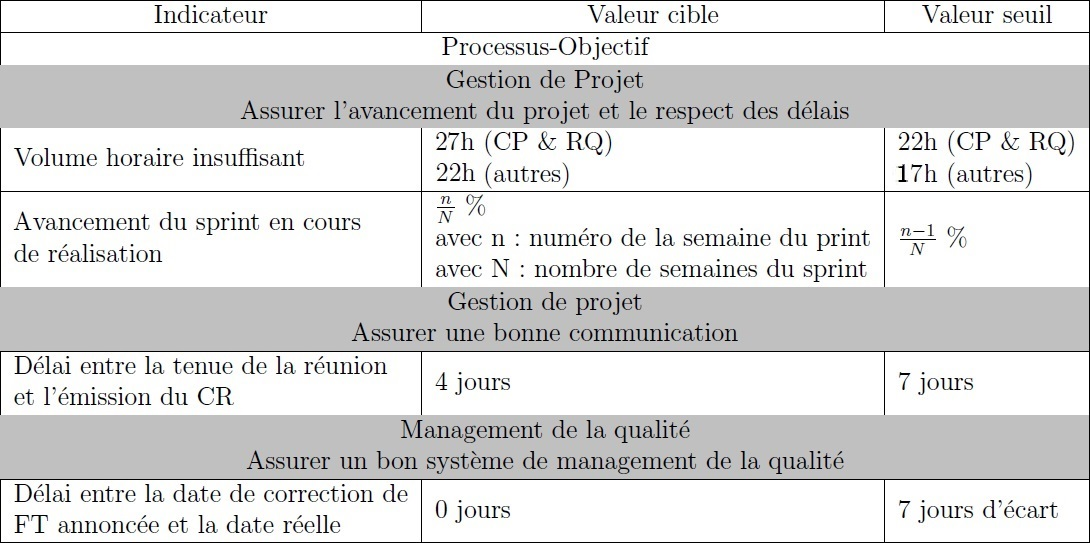
\includegraphics[width=13cm]{./images/indicateurs_hebdomadaires.jpg}
\end{figure}

\subsubsection*{Indicateurs ponctuels}
\label{Indicateurs ponctuels}
\paragraph*{} Les indicateurs ponctuels permettent de décrire les résultats d’événements ponctuels tels que les audits, les questionnaires de satisfaction, etc.

\paragraph*{} Un tableau récapitulant les indicateurs ponctuels mis en place est disponible dans le tableau
6.2. Pour les indicateurs faisant référence à des délais, le comptage exclut les vacances scolaires.
\begin{figure}[h]
   \center
   \caption{\label{Tableau 6.2} Indicateurs ponctuels}
   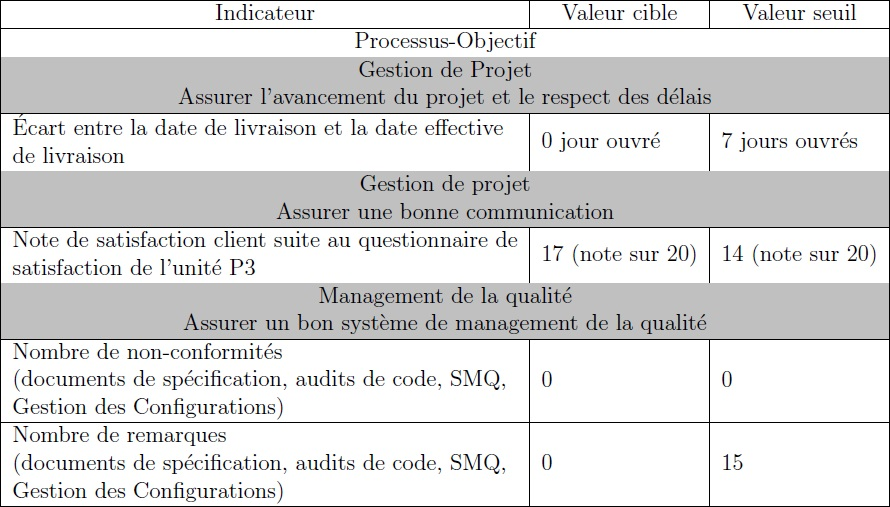
\includegraphics[width=13cm]{./images/indicateurs_ponctuels.jpg}
\end{figure}

\subsubsection*{Tableau de bord}
\label{Tableau de bord}

\paragraph*{} Le \TB{} est un outil de suivi qui permet à l'équipe \nomEquipe{} de suivre visuellement l'évolution de la qualité grâce à la représentation des différents états des indicateurs
hebdomadaires.

\paragraph*{} Le \RQ{} sera en charge de la mise à jour de ce document, à raison d'une
fois par semaine. Chaque \TB{} sera imprimé, attaché dans la salle PIC, archivé
numériquement dans le \DSQ{} et en version papier dans l'armoire de la salle.

\section{Suivi de la qualité}
\label{Suivi de la qualite}
\subsection{Surveillance de la qualité du code}
\label{Surveillance de la qualite du code}
\paragraph*{} La surveillance de la qualité du code sera exécutée tout au long de la phase de codage du
PIC par le \RD , notamment grâce à des outils de vérification de règles de codage.

\paragraph*{} Une vérification de code aura lieu toutes les deux semaines. Elle sera menée par le \RD . En cas de besoin, ce dernier peut déléguer cette tâche à un autre membre
du PIC.

\paragraph*{} Les rapports consécutifs à ces vérifications seront archivés une fois les tests exécutés. De plus, un audit sera programmé au besoin par l'unité P3.

\subsection{\FT}
\paragraph*{} Le système de traitement des Faits Techniques (\FTCourt) assure un bon suivi de la qualité dans
le PIC.

\paragraph*{} L'enregistrement d'un \FT{} sur \lintranet{} permet de faire constater qu'un écart ou
qu'une insatisfaction a été relevé. Il témoigne donc de l'enregistrement et de la prise en compte
du problème par l'équipe PIC.

\paragraph*{} Un \FTCourt{} est corrigé par un \OC{} (\OCCourt), lui aussi enregistré grâce à l'outil
\lintranet .

\subsubsection*{\FT}
\paragraph*{} Un \FT{} peut découler d'une remarque venant d'une source qui peut être :

\begin{itemize}
	\item le client (remarques, points à modifier...) ;
	\item l'équipe PIC (problèmes internes, de planning, ...) ;
	\item un audit PIC ;
	\item une inspection.
\end{itemize}

\paragraph*{} Un \FTCourt{} a une gravité qui peut être :
\begin{itemize}
\item mineure : n'implique aucun retard dans le déroulement du projet ;
\item gênante : peut retarder la tâche mais pas le projet ;
\item très gênante : risque fortement d'entraîner un retard dans le projet ;
\item bloquante : bloque le déroulement.
\end{itemize}

\paragraph*{} De même, un \FTCourt{} est caractérisé par un type qui peut être :
\begin{itemize}
\item anomalie ;
\item remarque ;
\item actualisation ;
\item demande d'évolution ;
\item demande de correction.
\end{itemize}

\paragraph*{} Un \FTCourt{} permet de faire état d'un écart. Si plusieurs écarts sont constatés dans un même
document, ceux-ci peuvent éventuellement être regroupés au sein d'un même \FTCourt . Ce \FTCourt{} sera
clôturé après clôture de l'\OCCourt{} correspondant. Chaque \OCCourt{} devra être vérifié.
\paragraph*{} Une action demandée par un \OCCourt{} peut être :
\begin{itemize}
\item préventive ;
\item corrective ;
\item curative.
\end{itemize}

\paragraph*{} On privilégiera la mise en place d'actions préventives dans le cas d'identification préalable
d'un risque et d'actions correctives dans le cas d'identification d'un problème avéré.


\subsubsection*{\CTFT (\CTFTCourt)}
\paragraph*{} Les \CTFTCourt{} auront lieu à intervalles réguliers et seront adaptables en fonction du nombre de \FTCourt{} à
traiter.

\paragraph*{} Une \CTFTCourt{} permet d'étudier les différentes \FTCourt{} en cours et est composée des personnes
suivantes :
\begin{itemize}
\item les auteurs des \FFTCourt{} dans la mesure du possible ;
\item les responsables de corrections si besoin ;
\item les vérificateurs ;
\item la personne en charge de la clôture des \OCCourt .
\end{itemize}

\subsubsection*{Cycle d'un \FTCourt}
Le cycle d'un \FTCourt{} est présenté dans la figure 6.3.

\begin{figure}[h]
   \center
   \caption{\label{Figure 6.1} Cycle d'un \FT}
   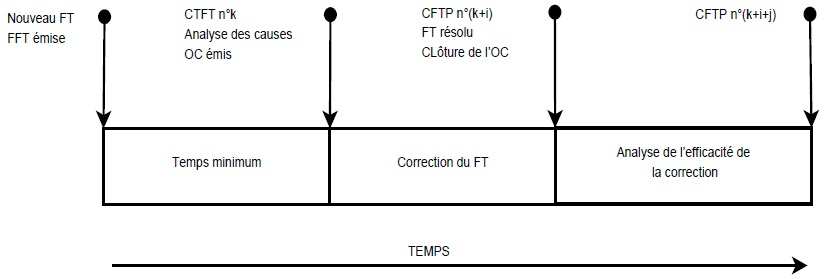
\includegraphics[width=13cm]{./images/cycle_d_un_fait_technique.jpg}
\end{figure}

\subsubsection*{\FTCourt{} relatifs aux documents soumis à l’approbation}
\paragraph*{} Les demandes de modification(s)/évolution(s)/correction(s) de documents soumis à approbation ne feront pas l'objet d'émission de \FTCourt{} si les dites modification(s)/évolution(s)/correction(s) ne concernent que la forme du document (orthographe, mise en page...).

\subsection{Audits internes}
\paragraph*{} Conformément à la Norme ISO 9001:2015 , des audits internes (un durant le premier semestre et un durant le second) seront menés pour évaluer le management de la Qualité au sein du PIC et déterminer si le \SMQCourt{} est conforme :
\begin{itemize}
\item aux exigences de la Norme ISO 9001:2015 ;
\item au \SMQ{} de l'Unité P3 du département \ASI ;
\item aux dispositions prises par la direction du PIC (engagements, \PQCourt , \PGCCourt).
\end{itemize}
\paragraph*{} La mise en place d'un tel audit consiste à vérifier que les dernières versions des documents
Qualité du PIC sont cohérentes et à jour ainsi qu'à effectuer une surveillance des configurations.
Toute remarque ou non-conformité fera l'objet d'une \FFTCourt .

\paragraph*{} Pour chaque audit, un enregistrement de l'audit et de ses résultats sera établi et conservé
puis une vérification sera faite dans le but de contrôler que la correction des éventuelles non-conformités a été faite dans le temps imparti.

 
\chapter{Vérification et validation}
\label{verification_et_validation}
% version 1.00	Auteur Kafui Atanley

Chaque document produit par le PIC doit faire l'objet d'une vérification, d'une validation
et d'une approbation avant diffusion. Ce cycle est présent et décrit dans le \PGC{} (\PGCCourt). Il est cependant rappelé ici de façon à faciliter la recherche d'informations le concernant.

\section{Vérification}
\label{Verification}

\subsubsection*{A faire avant de commencer la vérification}
Avant toute chose, il est nécessaire de vérifier sur la plate-forme installée sur le serveur
(\lintranet) que le rédacteur a bien signalé que la rédaction du document est terminée.

\subsubsection*{A faire pour la vérification}
Le vérificateur doit vérifier les points suivants :
\begin{itemize}
\item vérification orthographique du document ;
\item vérification de la mise en page ;
\item vérification du suivi du document.
\end{itemize}
Des commandes LATEX peuvent être mises en place par exemple dans le cas où le rédacteur
n'est pas sûr concernant un certain point. Ces commandes peuvent insérer des caractères dans le texte.
Le vérificateur devra vérifier qu'il n'y a plus d'insertion de ce type dans le document.

\subsubsection*{A faire après avoir effectué la vérification}

Après avoir vérifié un document, la personne en charge de cette tâche devra :
\begin{itemize}
\item le signaler sur \lintranet ;
\item signer le document papier si nécessaire ;
\item modifier le document numérique pour indiquer la date et indiquer qu'il a appliqué son
visa.
\end{itemize}

Le visa dans le document numérique peut être matérialisé de trois façons différentes :
\begin{itemize}
\item \lintranet : le visa est matérialisé seulement sur \lintranet{} par une case cochée.
\item Courriel : le visa a été matérialisé par courriel.
\item Signé : le visa a été matérialisé sur le document papier par une signature.
\end{itemize}

\subsection{Validation}
\label{Validation}

\subsubsection*{A faire avant de commencer la validation}
Le validateur doit s'assurer que le vérificateur a bien indiqué sur \lintranet{} et sur le document que le document en question est vérifié.

\subsubsection*{A faire pour la validation}
Le validateur doit valider les points suivants :
\begin{itemize}
\item la pertinence du document ;
\item la complétude du contenu par rapport aux objectifs fixés.
\end{itemize}

\subsubsection*{A faire après avoir effectué la validation}
Après avoir validé un document, la personne en charge de cette tâche devra :
\begin{itemize}
\item le signaler sur \lintranet ;
\item signer le document papier si nécessaire ;
\item modifier le document numérique pour indiquer la date et indiquer qu'il a appliqué son
visa.
\end{itemize}

Le visa dans le document numérique peut être matérialisé de trois façons différentes :
\begin{itemize}
\item \lintranet : le visa est matérialisé seulement sur \lintranet{} par une case cochée.
\item Courriel : le visa a été matérialisé par courriel.
\item Signé : le visa a été matérialisé sur le document papier par une signature.
\end{itemize}


\subsection{Approbation}
\label{Approbation}

Pour les documents qui ont une portée extérieure au PIC, une approbation sera nécessaire par la personne concernée extérieure au PIC. Le document une fois approuvé devient un enregistrement.

\subsubsection*{Approbation par les tuteurs}
Après chaque réunion avec un des tuteurs, un compte rendu ayant parcouru le cycle de
vérification et validation doit être approuvé.


\subsubsection*{Approbation par les tuteurs}
En ce qui concerne les documents approuvables par le client, si aucune remarque n'est effectuée
par le client sur le relevé de conclusions de réunions sous sept jours après l'envoi de ce dernier,
le compte-rendu est considéré comme approuvé.

\subsection{Diffusion}
\label{Diffusion}

Une fois approuvé (si le document nécessite une approbation), le document peut être diffusé.
Pour les documents sans approbation, c'est le rédacteur qui le diffuse. Pour le reste, c'est au
Chef PIC de s'en charger.

\section{Vérification et validation de lots}
\label{Vérification et validation de lots}

Pour certaines livraisons, il se peut que le lot soit un ensemble de documents. Dans ce cas,
le vérificateur doit vérifier que tous les documents sont présents.
\\
Ce vérificateur devra rédiger un \PVVV{} (\PVVVCourt).


\chapter{Procédures et description de mesure d'analyse, Amélioration SMQ}
\label{mesure_analyse_amelioration_SMQ}
\section{Procédures et déscription de mesure d'analyse et d'amélioration du SMQ}\label{qualite}

Concernant cette partie ainsi que la description de la procédure de traitement des faits techniques, se reporter à la partie "Procédures et description du management de la qualité" et "Procédures et description de la vérification, surveillance et validation des documents"


\chapter{Management des ressources du projet}
\label{ressources}
% version 1.00	Auteur Mathieu Médici

\section{Organisation} \label{Organisation}

L'organigramme visible en figure \ref{organigramme} ci-dessous présente les ressources humaines et leurs rôles principaux associés.

\begin{figure}[H]
   \centering
   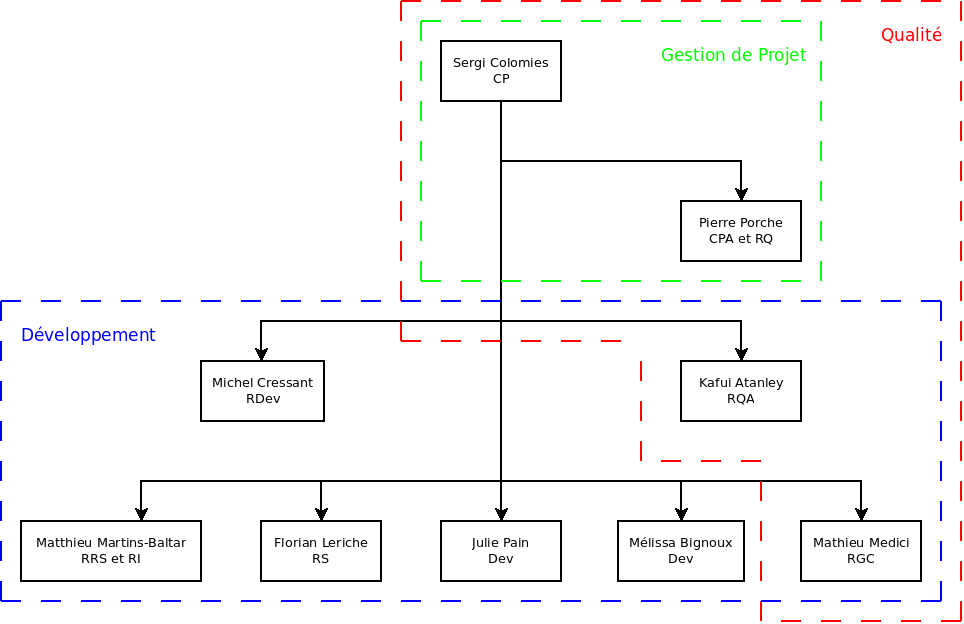
\includegraphics[width=15cm]{images/organigramme.png}
   \caption{\label{organigramme} Organigramme de \nomEquipe}
\end{figure}

\section{Compétences et formations} \label{CompetencesEtFormations}
\subsection{Rôles et compétences} \label{RolesEtCompetences}

\indent Chaque membre de l'équipe \nomEquipe{} est associé à un ou plusieurs rôles que l’on peut voir dans l’organigramme présenté ci-avant.\\

\indent Par défaut, chaque membre possède le rôle de Développeur. On lui ajoute ensuite un rôle spécifique si nécessaire. Il pourra se voir attribuer le rôle de Pilote de Risque ou Pilote d'Opportunité si celui-ci prend en charge la gestion d’un risque particulier ou d'une opportunité particulière.\\ 

\indent Le rôle de Responsable des Indicateurs sera également ajouté au Responsable Qualité, qui sera chargé de la mise à jour des indicateurs et du tableau de bord. \\

\indent Chaque attribution de rôle est justifiée par des compétences spécifiques que le titulaire doit posséder. C’est pourquoi les fiches de rôles spécifient les compétences requises pour effectuer une tâche. Ces fiches sont disponibles en annexe \ref{annexeFRo}. \\

\indent Ces Fiches de compétences, figurant dans le Dossier de Suivi de la Qualité, permettent de suivre le plan de formation de chaque membre de l’équipe PIC. Le formalisme d’une telle Fiche de compétences est disponible en annexe \ref{annexeFC}.\\

\indent Certaines personnes ont également des rôles plus particuliers détaillés dans la table \ref{repartRoles}. Chacun de ces rôles est défini dans une fiche de rôle disponible en annexe \ref{annexeFRo}.\\

\begin{table}[H]
\begin{tabular}[h]{|p{0.25\textwidth}|p{0.7\textwidth}|}
	\hline
	\rowcolor[gray]{0.85}
	Membre équipe PIC & Rôle(s) dans le projet \\\hline
	\Sergi &  \CP \\\hline
	\Pierre & \CPA, \RQ, \RI \\\hline
	\Kafui & \RQA, \D \\\hline
	\Mathieu & \RGC, \D \\\hline
	\Michel & \RD \\\hline
	\Matthieu & \RRS, \D \\\hline
	\Florian & \RS \\\hline	
	\Julie & \D \\\hline
	\Melissa & \D \\\hline
\end{tabular}
\caption{\label{repartRoles} Répartition des rôles}
\end{table}

\subsection{Formations} \label{formation}

Si l'un des titulaires d'une tâche n'a pas les compétences requises pour la réaliser, il doit suivre une formation. Cette formation peut être organisée par un professeur, un autre membre de l'équipe PIC ou une personne externe. Si aucune de ces solutions n'est envisageable, le titulaire pourra s'autoformer.\\

Le temps nécessaire à une formation fait partie du planning du PIC et celle-ci apparaîtra comme une tâche dans le planning. \\

Dans le cas où tous les membres du PIC devront s'autoformer à une technologie spécifique, deux membres du PIC devront réaliser un \QCM.

Un des deux \QCMCourt{} sera choisi pour que tous les membres du PIC soient évalués sauf le rédacteur de ce même \QCMCourt{} qui passera le second \QCMCourt.

Pour qu'une personne valide la formation, il faut que le \QCMCourt{} soit réussi à 66\% minimum. En cas d'échec à une évaluation, le membre devra se former de nouveau et repasser un \QCMCourt{} réalisé par un membre du PIC ayant obtenu cette compétence.

\section{Présence des membres}
\label{Présence des membres}

\subsection{Le temps de travail}
\label{temps_de_travail}
Selon le contrat d'étude, chaque membre de l'équipe doit faire un total de 22 heures de travail par semaine comprenant cinq jours ouvrés sur le \PICCourt. Le \CP{} et le \RQ{} possédant deux crédits de plus chacun, ils devront effectuer 27 heures par semaine comprenant cinq jours ouvrés. Si un ou quelques jours parmi ces cinq jours ouvrés sont fériés ou banalisés, on retire du volume horaire attendu les heures réservées à la réalisation du PIC sur ces jours fériés ou banalisés.

\subsection{En salle PIC}
\label{en_salle_pic}
Pour chaque membre, il est obligatoire de travailler au minimum 17 heures en salle PIC par semaine comprenant cinq jours ouvrés. Pour le \CP{} et le \RQ{} ce temps est de 22 heures par semaine comprenant cinq jours ouvrés. Si un ou quelques jours parmi ces cinq jours ouvrés sont fériés ou banalisés, on retire du volume horaire attendu les heures réservées à la réalisation du PIC sur ces jours fériés ou banalisés.\\

Un planning détaillé recensant les heures en salle de chaque membre sera créé et affiché.
Ce planning sera un moyen pour que le \CP{} estime les ressources humaines disponibles à n'importe quel moment de la semaine.

\section{Locaux de réalisation du projet}
\label{Locaux de réalisation du projet}
\indent L'INSA, et plus précisément le département \ASI{}, met à disposition de chaque équipe une salle de travail située dans le bâtiment Bougainville. Chaque équipe \PIC{} bénéficie de cette salle pour toute la durée du projet.
Concernant notre équipe, \nomEquipe, la salle qui nous a été attribuée est ARC04.

\section{Inventaire du matériel mis à disposition}
\label{Inventaire du matériel mis à disposition}
Notre salle \PICCourt a été fournie avec du matériel informatique dont l'inventaire est le suivant : Annexe \ref{annexeInventaire}.

\section{Inventaire des ressources informatiques}
\label{Inventaire des ressources informatiques}
Les ressources mises à disposition par le département \ASI{} pour l'équipe Unipik sont :

\begin{itemize}
	\item Un dépôt \git{} sur la plate-forme MonProjet de l'INSA de Rouen;
	\item Un logiciel de gestion de projet: PGPic.\\
\end{itemize}

Cependant, il est possible que d'autres logiciels soient utilisés par l'équipe PIC tout au long du projet à condition que ceux-ci soient libres de droit d'utilisation.

\section{Matériel à acheter}
\label{Matériel à acheter}
\indent Un budget de 700 euros a été défini concernant le projet. Cependant l'application doit être le plus proche possible de la gratuité (utilisation de logiciels et technologies issus du monde libre). \\
\indent Le secrétariat du département tient à jour un tableur où sont stockés les suivis de budget de toutes les équipes PIC.

\section{Eventuelle licence informatique à commander}
\label{Eventuelle licence informatique à commander}
\indent Pour le moment aucun achat de licence n'est nécessaire au projet.

\section{Matériel et/ou logiciel fournis par le client}
\label{Matériel et/ou logiciel fournis par le client}
\indent Pour le moment aucun prêt de matériel et/ou logiciel n'a été fait par le client.\\
\indent Dans le cas où des données seraient fournies à l’équipe \PICCourt par le client, il faut faire une \FEDC. A la fin du PIC, la \FEDCCourt certifie de la destruction des données.

\section{Description des procédures relatives à l'écoute client}
\label{DescrProceduresRelativesALecouteClient}
\indent La communication avec le client devra s'effectuer de manière méthodique à travers les revues de \DSI{} (\DSICourt), \DSE{} (\DSECourt) et de fin de phase de \PICCourt. Dans ces revues, les attentes du client seront prises en compte afin de satisfaire ses besoins au maximum (cf Partie \ref{specification} - \PQCourt). Des réunions régulières devront également être réalisées ainsi qu'un \CRC{} après chaque réunion. Celui-ci devra être validé par le client afin d'éviter les incompréhensions entre les deux partis. \\
Le client pourra faire des remarques (observations) et des réclamations, c'est-à-dire exprimer son mécontentement concernant le produit, service ou le processus de traitement des réclamations lui-même, pour laquelle une réponse ou une solution est explicitement ou implicitement attendue (cf Partie 3.1 - \MQ). 
Les procédures à effectuer lors d'une réclamation ou une remarque du client devront être différenciées et sont décrites dans les parties suivantes.
   
\subsection{Remarques du client}
\label{RqClient}
A chaque remarque faite du client, une \FFT{} devra être rédigée (voir Annexe \ref{fft}).

\subsection{Réclamations du client}
\label{ReclamClient}
Une attention particulière est apportée au suivi des réclamations client. En effet, à chaque réclamation de la part de ce dernier, une \FFT{} (voir Annexe \ref{fft}) devra également être réalisée et un email devra être envoyé au client. 


 
\begin{appendix}
\part*{Annexes}
\addcontentsline{toc}{part}{Annexes}

\chapter{Check-list de Vérification}
\label{annexeCheckList}
% version 1.00	Auteur Mélissa Bignoux

\begin{table}[H]
\centering
 \begin{tabular}{|l | c|}
 \hline
 \cellcolor{gray!40} Vérifier les pages de service & $\square$ \\
 \hline
  ~~Vérifier les dates du document & $\square$ \\
  ~~Vérifier les dates de suivi de diffusion & $\square$ \\
  ~~Vérifier la correction des FFT correspondantes & $\square$ \\
  ~~Vérifier la présence d'un tableau de définitions & $\square$ \\
  ~~Vérifier la présence d'un tableau d'abréviations & $\square$ \\
  ~~Vérifier le mode de diffusion & $\square$ \\
  \hline
 \cellcolor{gray!40} Respect de la langue française & $\square$ \\
 \hline
  ~~Fautes de français & $\square$ \\
  ~~Vérification de la ponctuation & $\square$ \\
  ~~Concordance du formalisme des listes & $\square$ \\
 \hline
 \cellcolor{gray!40} Structure et mise en page du document & $\square$ \\
 \hline
  ~~Vérification de la présence de la légende pour les figures & $\square$ \\
  ~~Vérification de la présence de la légende pour les tableaux & $\square$ \\
  ~~Cohérence dans la numérotation des parties du document & $\square$ \\
  ~~Cohérence des références & $\square$ \\
  ~~Vérifier la présence d'une liste des figures et d'une liste des tableaux & $\square$ \\
  \hline
  \cellcolor{gray!40} Vérifier l'adéquation des fichiers avec le PGC  & $\square$ \\
  \hline
 \end{tabular}
\end{table}




\chapter{Exemple de Portefeuille de Risques et d'Opportunités}
% version 2.00	Auteur Pierre Porche


\section*{Tableaux de suivi}


\subsection*{Suivi des Risques}
\begin{longtable}{|p{0.3cm}|p{2.5cm}|p{2cm}|p{2cm}|p{1.8cm}|p{1.5cm}|p{1cm}|p{1cm}|p{1.5cm}|}
			\hline
			\rowcolor{gray!40}
			\No & Nom & Pilote & Probabilité & Impact & Priorité & Visa \RQCourt{} & Visa \CPCourt{} & Clôture \\\hline
			
			 1 & Risque 1 & Un nom & Une probabilité & Un impact & Une priorité & Un visa & Un visa & \\\hline
			 
			 2 & Risque 2 & Un autre nom & Une autre probabilité & Un autre impact & Une autre priorité & Un visa & Un visa & Clôturé \\\hline
			 
			 
\end{longtable}

\subsection*{Suivi des Opportunités}

\begin{longtable}{|p{0.3cm}|p{2.5cm}|p{2cm}|p{2cm}|p{1.8cm}|p{1.5cm}|p{1cm}|p{1cm}|p{1.5cm}|}
			\hline
			\rowcolor{gray!40}
			\No & Nom & Pilote & Probabilité & Impact & Priorité & Visa \RQCourt{} & Visa \CPCourt{} & Clôture \\\hline
			 
			 1 & Opportunité 1 & Un nom & Une probabilité & Un impact & Une priorité & Un visa & Un visa & \\\hline
			 
			 2 & Opportunité 2 & Un autre nom & Une autre probabilité & Un autre impact & Une autre priorité & Un visa & Un visa & Clôturé \\\hline
			 			 
\end{longtable}

\newpage

\label{annexeFRi}
% version 1.00	Auteur Julie Pain

\section*{Informations générales}
 
\begin{table}[H]
\centering
	\begin{tabularx}{16.8cm}{|X|X|}
	\hline
	\rowcolor{gray!40} Numéro du risque & Type du risque \\
	\hline
	 &  \\
	\hline
	\end{tabularx}
\end{table}

\begin{table}[H]
\centering
	\begin{tabularx}{16.8cm}{|X|X|X|}
	\hline
	\rowcolor{gray!40} Date & Visa du \RQ & Visa du \CP \\
	\hline
	  & & \\
	\hline
	\end{tabularx}
\end{table}

\begin{table}[H]
\centering
	\begin{tabularx}{16.8cm}{|X|X|X|X|}
	\hline
	\rowcolor{gray!40} Pilote & Activité WBS & Compte WBS & Phase d'apparition \\
	\hline
	  & & &\\
	\hline
	\end{tabularx}
\end{table}

\section*{Description du risque}

\subsection*{Résumé}
	Indiquer ici un résumé du risque.
	
\subsection*{Analyse des causes}
	Inclure ici un graphique issu de la méthode des n pourquoi afin d'identifier les différentes causes.

\subsection*{Criticité}

\begin{table}[H]
\centering
	\begin{tabularx}{16.8cm}{|>{\columncolor{gray!40}}X|X|}
	\hline
	Gravité & \\
	\hline
	Probabilité & \\
	\hline
	Criticité & \\
	\hline
	\end{tabularx}
\end{table}

\section*{Actions}
\subsection*{Actions préventives}

\begin{table}[H]
\centering
	\begin{tabularx}{16.8cm}{|X|X|}
	\hline
	\rowcolor{gray!40} Numéro de cause & Actions préventives \\
	\hline
	  & \\
	\hline
	\end{tabularx}
\end{table}

\subsection*{Plan de contournement}
Lister ici les différents plans de contournement permettant de contourner le risque.

\section*{Décision de clôture}
Par le \CP{} et le pilote du risque.
\begin{table}[H]
\centering
	\begin{tabularx}{16.8cm}{|X|X|}
	\hline
	\rowcolor{gray!40} Date de clôture & Raison de la clôture \\
	\hline
	  & \\
	\hline
	\end{tabularx}
\end{table}

\section*{Historique des modifications}
\begin{table}[H]
\centering
	\begin{tabularx}{16.8cm}{|X|X|}
	\hline
	Date & Modification \\
	\hline
	  & \\
	\hline
	\end{tabularx}
\end{table}
\newpage
\label{annexeFO}
% version 1.00	Auteur Pierre Porche

\section*{Informations générales}
 
\begin{table}[H]
\centering
	\begin{tabularx}{16.8cm}{|X|X|}
	\hline
	\rowcolor{gray!40} Numéro de l'opportunité & Type de l'opportunité \\
	\hline
	 &  \\
	\hline
	\end{tabularx}
\end{table}

\begin{table}[H]
\centering
	\begin{tabularx}{16.8cm}{|X|X|X|}
	\hline
	\rowcolor{gray!40} Date & Visa du \RQ & Visa du \CP \\
	\hline
	  & & \\
	\hline
	\end{tabularx}
\end{table}

\begin{table}[H]
\centering
	\begin{tabularx}{16.8cm}{|X|X|X|X|}
	\hline
	\rowcolor{gray!40} Pilote & Activité WBS & Compte WBS & Phase d'apparition \\
	\hline
	  & & &\\
	\hline
	\end{tabularx}
\end{table}

\section*{Description de l'opportunité}

\subsection*{Résumé}
	Indiquer ici un résumé de l'opportunité.
	
\subsection*{Analyse des causes}
	Inclure ici un graphique issu de la méthode des n pourquoi afin d'identifier les différentes causes.

\subsection*{Criticité}

\begin{table}[H]
\centering
	\begin{tabularx}{16.8cm}{|>{\columncolor{gray!40}}X|X|}
	\hline
	Bénéfice & \\
	\hline
	Probabilité & \\
	\hline
	Criticité & \\
	\hline
	\end{tabularx}
\end{table}

\section*{Actions}
\subsection*{Actions proactives}

\begin{table}[H]
\centering
	\begin{tabularx}{16.8cm}{|X|X|}
	\hline
	\rowcolor{gray!40} Numéro de cause & Actions proactives \\
	\hline
	  & \\
	\hline
	\end{tabularx}
\end{table}

\newpage


\chapter{Fiche de Fait Technique}
\label{annexeFFT}
% version 1.00	Auteur Pierre Porche

\section*{Identification du \FTCourt}
\label{fft}
\begin{table}[H]
\centering
	\begin{tabularx}{16.8cm}{|>{\columncolor{gray!40}}l|X|}
	\hline
	Numéro de référence & \\
	\hline
	Identification du document (contenant le code \PICCourt{}) & \\
	\hline
	Date de création & \\
	\hline
	Type de \FTCourt* & \\
	\hline
	Prénom et Nom de l'auteur & \\
	\hline
	Source du \FTCourt** & \\
	\hline
	\end{tabularx}
\end{table}
\noindent \small * Anomalie, Remarque, Non-conformité, Actualisation, Demande d'évolution ou Demande de correction. \\
\small ** Audit \PICCourt{}, Inspection, Réclamation client ou interne.

\section*{Documents en référence}

\begin{table}[H]
\centering
	\begin{tabularx}{16.8cm}{|>{\columncolor{gray!40}}l|X|}
	\hline
	Référence et version de l'objet du \FTCourt & \\
	\hline
	Référence de la \CTFTCourt & \\
	\hline
	Référence à l'\OC & \\
	\hline
	Description & \\
	\hline
	Gravité* & \\
	\hline
	\end{tabularx}
\end{table}
\noindent \small * Sans conséquence, grave ou très grave.

\section*{Analyse des causes}

Quelle est la cause du \FT ? (méthode des n pourquoi)
\begin{itemize}
	\item
	\item
	\item
\end{itemize}

\section*{Clôture de la \FFTCourt}

\begin{table}[H]
\centering
	\begin{tabularx}{16.8cm}{|>{\columncolor{gray!40}}l|X|}
	\hline
	Référence de la \CTFTCourt & \\
	\hline
	Prénom et Nom & \\
	\hline
	Date & \\
	\hline
	Signature & \\
	\hline
	\end{tabularx}
\end{table}

\section*{Analyse à froid}

\begin{table}[H]
\centering
	\begin{tabularx}{16.8cm}{|>{\columncolor{gray!40}}l|X|}
	\hline
	Date de l'analyse & \\
	\hline
	Prénom(s) et nom(s) & \\
	\hline
	Avis sur l'efficacité de la ou des correction(s) & \\
	\hline
	Observations si correction(s) non efficace(s) & \\
	\hline
	\end{tabularx}
\end{table}

\chapter{Fiche de Commission de Traitement des Faits Techniques}
\label{annexeFCTFT}
% version 1.00	Auteur Pierre Porche

\begin{table}[H]
\centering
	\begin{tabularx}{16.8cm}{|>{\columncolor{gray!40}}l|X|}
	\hline
	Date de réunion de la CTFT &  \\
	\hline
	\end{tabularx}
\end{table}


\begin{center}
	Membres de la CTFT
\end{center}
\begin{table}[H]
\centering
	\begin{tabularx}{16.8cm}{|X|X|X|X|}
	\hline
	
	\cellcolor{gray!40} NOM & 
	\cellcolor{gray!40} PRENOM & 
	\cellcolor{gray!40} FONCTION & 
	\cellcolor{gray!40} Signature \\
	
	\hline
	 & & & \\
	\hline
	& & & \\
	\hline
	
	\end{tabularx}
\end{table}



\begin{table}[H]
\centering
	\begin{tabularx}{16.8cm}{|X|X|X|}
	\hline
	
	 \cellcolor{gray!40} Numéro FFT analysée & 
	 \cellcolor{gray!40} Date d'émission du FT &
	 \cellcolor{gray!40} Date de clôture du FT \\
	
	\hline
	 & &  \\
	\hline
	& &  \\
	\hline
	
	\end{tabularx}
\end{table}


\begin{center}
	Analyse des FFT émises
\end{center}


\begin{table}[H]
\centering
	\begin{tabularx}{16.8cm}{|X|X|X|}
	\hline
	
	 \cellcolor{gray!40} Numéro de fiche d'Ordre de Correction & 
	 \cellcolor{gray!40} Numéro(s) du(des) FFT concernée(s) & 
	 \cellcolor{gray!40} Date limite de correction \\
	
	\hline
	 & &  \\
	\hline
	
	
	\end{tabularx}
\end{table}

\begin{center}
	Rédaction d'Ordre de Correction au regard de l'analyse des FT
\end{center}



\begin{table}[H]
\centering
	\begin{tabularx}{16.8cm}{|X|X|X|X|X|}
	\hline
	
	 \cellcolor{gray!40} Numéro FFT &
	 \cellcolor{gray!40} Numéro OC &
	 \cellcolor{gray!40} Le délai entre l'émission du FT et son OC ne dépasse pas 10j ouvrés (OUI/NON) &
	 \cellcolor{gray!40} Le délai entre l'émission de l'OC et sa prise en compte ne dépasse pas 2j ouvrés (OUI/NON) &
	 \cellcolor{gray!40} La délai entre la date d'émission du FT et sa clôture ne dépasse pas trois semaines (OUI/NON)  \\
	
	\hline
	 & & & & \\
	\hline
	 & & & & \\
	\hline
	 & & & & \\
	\hline
	
	
	\end{tabularx}
\end{table}

\begin{center}
	Respect des délais
\end{center}


\chapter{Fiche d'Ordre de Correction}
\label{annexeFOC}
% version 1.00	Auteur Pierre Porche

\section*{Identifiant}

\begin{table}[H]
\centering
	\begin{tabularx}{16.8cm}{|>{\columncolor{gray!40}}l|X|}
	\hline
	Numéro de référence & \\
	\hline
	Identification du document (contenant le code \PICCourt) & \\
	\hline
	Date de création & \\
	\hline
	Date limite de correction & \\
	\hline
	Auteur & \\
	\hline
	Correcteur & \\
	\hline
	Fonction du correcteur & \\
	\hline
	Vérificateur & \\
	\hline
	\end{tabularx}
\end{table}

\section*{FFT concernée(s)}

\begin{table}[H]
\centering
	\begin{tabularx}{16.8cm}{|X|X|X|}
	\hline
	\rowcolor{gray!40} \FFTCourt{} concernée(s) & Type d'action* & Description de la correction à apporter \\
	\hline
	 & & \\
	\hline
	\end{tabularx}
\end{table}
\noindent \small * Corrective ou Préventive

\section*{Articles ouverts à la correction}

\begin{table}[H]
\centering
	\begin{tabularx}{16.8cm}{|X|X|X|}
	\hline
	\rowcolor{gray!40} Nom de l'article & Référence & Version après correction \\
	\hline
	 & & \\
	\hline
	\end{tabularx}
\end{table}

\section*{Vérification}

\begin{table}[H]
\centering
	\begin{tabularx}{16.8cm}{|>{\columncolor{gray!40}}l|X|}
	\hline
	Prénom et Nom & \\
	\hline
	Date de la vérification & \\
	\hline
	Avis* & \\
	\hline
	Signature & \\
	\hline
	\end{tabularx}
\end{table}
\noindent \small * Satisfaisant ou Insatisfaisant

\section*{Clôture}

Un \OCCourt{} sur un document soumis à approbation ne peut être clôturé sans que celui-ci ait été réapprouvé au préalable.

\begin{table}[H]
\centering
	\begin{tabularx}{16.8cm}{|>{\columncolor{gray!40}}l|X|}
	\hline
	Prénom et Nom & \\
	\hline
	Date de la clôture & \\
	\hline
	Signature & \\
	\hline
	\end{tabularx}
\end{table}

\chapter{Fiches de Rôle}
\label{annexeFRo}
\section{\CP}
\subsection*{Introduction}

<<<<<<< HEAD
Le \CP{} doit garantir le bon déroulement du \PICCourt. Il possède des missions d’organisation et de validation du travail effectué par les membres de l’équipe. Il est également l’interlocuteur privilégié du tuteur pédagogique, du tuteur qualité et du client.
=======
Le \CP{} doit garantir le bon déroulement du \PICCourt. Il possède des missions d’organisation et de validation du travail effectué par les membres de l’équipe. Il est également l’interlocuteur privilégié du Tuteur Pédagogique, du Tuteur Qualité et du client.
>>>>>>> 0df4c754161dfe55442977f5cea6b2c3513bd81b

\subsection*{Tâches liées à sa fonction}

Une passation devra être mise en place entre les \CPs{} du premier et second semestre. Cette passation devra si possible être formalisée sous la forme d’une formation.

\subsection*{Tâches effectuées au démarrage du \PICCourt}

Le \CP{} devra se conformer aux exigences de la période de démarrage du \PICCourt :
\begin{itemize}
	\item Organiser l’équipe \PICCourt au premier semestre et de la fin du premier au second semestre en tenant compte des éventuels départs à l’étranger, redoublements, réorientations ou retours de mobilité académique. Ainsi qu’organiser la formation en début du second semestre du \PICCourt
<<<<<<< HEAD
	\item Créer le dépôt \git{} sur https://monprojet.insa-rouen.fr et des espaces publics et privés des membres de l’équipe \PICCourt
=======
	\item Créer le dépôt \git sur https://monprojet.insa-rouen.fr et des espaces publics et privés des membres de l’équipe \PICCourt
>>>>>>> 0df4c754161dfe55442977f5cea6b2c3513bd81b
	\item Rédiger ou faire rédiger, puis valider les \FC{} de son équipe et éventuellement attester certaines compétences d’ordre personnel.
	\item Établir l’organigramme des fonctions de son \PICCourt et les descriptifs de ces fonctions.
	\item Associer les ressources aux fonctions de son \PICCourt.
\end{itemize}

\subsection*{Tâches effectuées au cours du \PICCourt}

Le \CP{} devra remplir au cours du \PICCourt les missions suivantes :

\begin{itemize}
	\item Mettre à jour les \FC{} des membres du \PICCourt.
	\item Archiver de manière hebdomadaire l’ensemble des espaces privés des membres et les conserver sur clé USB jusqu’à la semaine suivante.
	\item Garantir les journaux de tests.
	\item Participer à la \CTFT (CTFT).
	\item Gérer le budget de fonctionnement du \PICCourt.
<<<<<<< HEAD
	\item Représenter les ressources globales du \PICCourt et le solde des ressources consommées par un \WBSCourt minimal, un OBS, un \RBSCourt{} ou un \FBSCourt.
=======
	\item Représenter les ressources globales du \PICCourt et le solde des ressources consommées par un \WBSCourt{} minimal, un OBS, un \RBSCourt{} ou un \FBSCourt.
>>>>>>> 0df4c754161dfe55442977f5cea6b2c3513bd81b
	\item Collecter les risques de tâches mis en lumière par les membres de l’équipe.
	\item Participer à la réunion de la conduite de projet ou suivi prévisionnel tenue au minimum une fois par semestre.
	\item Effectuer le débriefing à la revue de \PICCourt.
	\item Accorder les dérogations de possibilité de diffusion des non-conformités en accord avec le client.
\end{itemize}

Le \CP{} devra également remplir ou déléguer ces missions au \CPA :
\begin{itemize}
	\item Animer la réunion d’avancement hebdomadaire.
	\item Établir les diagrammes de Gantt pour le suivi des tâches passées, en cours et futures.
	\item Reprendre le planning de la semaine passée et le mettre à jour en fonction des retards estimés, des réunions exceptionnelles et des corrections possibles.
	\item Vérifier les fiches de suivi hebdomadaire des membres de l’équipe.
\end{itemize}

\subsection*{Tâches effectuées en fin de période du \PICCourt}

Le \CP{} devra en fin de période remplir les missions suivantes :
\begin{itemize}
	\item Livrer au secrétariat de la Direction du Département \ASICourt{} l’archivage de l’espace public des membres de l’équipe en fin de semestre.
	\item Garantir avec la Direction Qualité dans un \PVCourt{} la fin de la phase d’intégration.
\end{itemize}
\newpage

\section{\CPA}
\subsection*{Introduction}

<<<<<<< HEAD
Durant le premier semestre, le \CPA{} doit seconder le \CP{} et effectuer les tâches qu’il lui aura délégué. À la fin de ce semestre, dans la majorité des cas, il devra se préparer à assurer le rôle de \CP.
=======
Durant le premier semestre, le \CPA{} doit seconder le \CP{} et effectuer les tâches qu’il lui aura déléguées. À la fin de ce semestre, dans la majorité des cas, il devra se préparer à assurer le rôle de \CP.
>>>>>>> 0df4c754161dfe55442977f5cea6b2c3513bd81b

\subsection*{Tâches liées à sa fonction}

Le \CPA{} devra remplir les missions suivantes :
\begin{itemize}
	\item Établir avec le \CP{} le planning détaillé des activités à réaliser ;
	\item Réaliser avec le \CP{} le suivi du projet ;
	\item Remplacer le \CP{} si celui-ci est indisponible ;
<<<<<<< HEAD
	\item Préparer le semestre suivant, en collaboration avec le \CP, à la fin du premier semestre, s’il prend la fonction de \CP{} au second semestre.
=======
	\item Préparer le semestre suivant, en collaboration avec le \CP{}, à la fin du premier semestre, s’il prend la fonction de \CP{} au second semestre.
>>>>>>> 0df4c754161dfe55442977f5cea6b2c3513bd81b
\end{itemize}

\newpage
\section{\RQ}
\subsection*{Introduction}

Le \RQ{} est le garant de l’application de la politique qualité au sein du \PICCourt. Il peut être épaulé dans cette tâche par d’autres membres du \PICCourt.

\subsection*{Tâches liées à sa fonction}

Une passation devra être mise en place entre les \RQs{} du premier et second semestre. Cette passation devra si possible être formalisée sous la forme d’une formation.\\
Tout au long du projet, le \RQ{} devra veiller à la bonne adéquation entre les tâches liées à la réalisation des livrables et le référentiel qualité. Pour assurer le bon déroulement de cette veille qualité, il devra réaliser les tâches suivantes :

\subsubsection*{Tâches liées au \PQCourt}
\begin{itemize}
<<<<<<< HEAD
	\item Rédiger et organiser le suivi du \PQ (\PQCourt) en respectant les exigences du Référentiel Qualité et en particulier de la \DGQDEUXCourt.
	\item Assurer la bonne diffusion (c’est à dire, l’envoi après approbation) du \PQCourt{} aux membres de l’équipe \PICCourt.
	\item Vérifier le \PQCourt{} après l’exécution d’actions correctives (cette tâche peut être déléguée à un autre membre du \PICCourt par dérogation personnelle ou de la part du \CP).
=======
	\item Rédiger et organiser le suivi du \PQ{} (\PQCourt) en respectant les exigences du Référentiel Qualité et en particulier de la \DGQDEUXCourt.
	\item Assurer la bonne diffusion (c’est à dire, l’envoi après approbation) du \PQCourt{} aux membres de l’équipe \PICCourt.
	\item Vérifier le \PQCourt{} après l’exécution d’actions correctives (cette tâche peut être déléguée à un autre membre du \PICCourt{} par dérogation personnelle ou de la part du \CP).
>>>>>>> 0df4c754161dfe55442977f5cea6b2c3513bd81b
	\item Valider l’ensemble des procédures qualité rédigées au sein du \PICCourt.
	\item Fournir un accompagnement aux équipes de développement dans la démarche qualité.
	\item Réaliser des activités régulières de contrôle de l’ensemble du système qualité.
	\item Sensibiliser les membres de l’équipe \PICCourt{} à la norme \ISOCourt 9001:2015.
\end{itemize}

\subsubsection*{Tâches liées au \PGCCourt}

Cette partie peut être déléguée dès le début du \PICCourt{} à un autre membre du \PICCourt{}, possédant la compétence exigée, qui prendra alors la responsabilité de la gestion des configurations.

\begin{itemize}
	\item Rédiger et organiser le suivi du \PGCCourt{} en respectant les exigences du Référentiel Qualité et en particulier de la \DGQDEUXCourt.
<<<<<<< HEAD
	\item Vérifier le \PGCCourt après l’éxécution d’actions correctives (cette tâche peut être déléguée à un autre membre du \PICCourt par dérogation personnelle ou de la part du \CP).
=======
	\item Vérifier le \PGCCourt{} après l’exécution d’actions correctives (cette tâche peut être déléguée à un autre membre du \PICCourt{} par dérogation personnelle ou de la part du \CP).
>>>>>>> 0df4c754161dfe55442977f5cea6b2c3513bd81b
	\item Garantir l’application du \PGCCourt.
	\item S’assurer du bon déroulement de la gestion des modifications des différents documents.
\end{itemize}

\subsubsection*{Tâches liées à la gestion du référentiel}

\begin{itemize}
<<<<<<< HEAD
	\item Chaque semestre, les \RQs{} doivent se réunir et fournir au pilote de processus 2, une liste de cinq questions par responsable visant à évaluer la maîtrise de ce référentiel ;
=======
	\item Chaque semestre, les \RQs{} doivent se réunir et fournir au pilote de processus 2, une liste de 5 questions par responsable visant à évaluer la maîtrise de ce référentiel ;
>>>>>>> 0df4c754161dfe55442977f5cea6b2c3513bd81b
	\item Chaque semestre, les \RQs{} doivent se réunir pour se répartir et corriger les demandes d’amélioration présentes sur l’outil de suivi des référentiels ;
	\item Chaque semestre, à chaque incohérence et problème soulevé, les \RQs{} doivent ajouter des demandes d’amélioration à l’aide de l’outil de suivi des référentiels.
\end{itemize}

\newpage
\section{\RQA}
\subsection*{Introduction}

Durant le premier semestre, le \RQA{} doit seconder le \RQ{} et effectuer les tâches qu’il lui aura déléguées. À la fin de ce semestre, dans la majorité des cas, il devra se préparer à assurer le rôle de \RQ .

\subsection*{Tâches liées à sa fonction}

Le \RQA{} devra remplir les missions suivantes :
\begin{itemize}
	\item Tenir à jour les différents indicateurs mis en place pour le \PICCourt.
	\item Remplacer le \RQA{} si celui-ci est indisponible ;
	\item Seconder le \RQ{} dans la réalisation du \PQ, du \PGC{} ainsi que des autres documents liés au projet.
        \item Participer au développement des fonctionnalités nécessaires au projet. 
\end{itemize}

\newpage
\section{\RGC}
\subsection*{Introduction}

Au début du projet, le \RGC{} doit s'occuper de la rédaction du \PGCCourt{} qui sert à contrôler l’activité de gestion des configurations pendant toute la durée du \PICCourt. L’élaboration de ce document permet donc de fixer toutes les règles de la gestion des configurations. Ce dernier sera amené à évoluer tout au long du projet afin que cette gestion soit toujours adaptée au \PICCourt.

\subsection*{Tâches liées à sa fonction}

Le \RGC{} devra remplir les missions suivantes :
\begin{itemize}
	\item Mettre en place le gestionnaire de sources du \PICCourt.
	\item Rédiger le \PGC.
	\item Fixer les règles de la gestion des configurations.
        \item Clôturer les ordres de corrections après avoir vérifié que la procédure de correction/vérification avait bien été respectée.
        \item Se charger de l'effacement du dépôt des sources.
        \item S'assurer que les membres de l'équipe \PICCourt{} respectent le \PGCCourt.
\end{itemize}

\newpage
\section{\RRS}
\subsection*{Introduction}

Au début du projet, le \RRS{} doit s'occuper de la mise en place du réseau dans la salle \PICCourt afin que chaque membre ait accès à internet et puisse travailler dans de bonnes conditions. Il sera chargé de maintenir ce réseau fonctionnel tout au long du projet.

\subsection*{Tâches liées à sa fonction}

Le \RRS{} devra remplir les missions suivantes :
\begin{itemize}
	\item Mettre en place le réseau en salle \PICCourt.
	\item S'assurer du bon fonctionnement du réseau tout au long du \PICCourt.
	\item S'assurer du bon état de fonctionnement du serveur.
	\item Faire évoluer l'architecture du réseau en fonction des besoins utilisateurs.
	\item Participer à la gestion technique des équipements. Cela consiste à réceptionner les matériels informatiques et de télécommunications, les tester, les adapter, les insérer dans le réseau en fonctionnement et effectuer le suivi du parc de matériels.
\end{itemize}

\newpage
\section{\RD}
\subsection*{Introduction}

Tout au long du projet, le \RD{} doit s'occuper de la gestion de toutes les parties concernant le développement. Il aura donc sous sa charge un certain nombre de développeurs et va devoir s'assurer que les résultats issus du développement sont conformes au \DGQDEUXCourt.

\subsection*{Tâches liées à sa fonction}

Le \RD{} devra remplir les missions suivantes :
\begin{itemize}
	\item Définir avec le \CP{} les différentes phases de conception et de développement.
	\item Établir les phases de vérification et de validation du développement.
<<<<<<< HEAD
	\item Participer à la réalisation du \DSECourt, du \DSICourt{} et du \PTVCourt.
=======
	\item Participer à la réalisation du \DSECourt{}, du \DSICourt{} et du \PTVCourt.
>>>>>>> 0df4c754161dfe55442977f5cea6b2c3513bd81b
	\item S'assurer de la réussite des tests unitaires et d'intégration.
	\item S'assurer que les codes fournis fonctionneront également chez le client.
\end{itemize}	

\chapter{Fiche de Compétences}
\label{annexeFC}
\documentclass[11pt]{article}
\usepackage{draftcopy}
\usepackage[francais]{babel}
\usepackage[utf8]{inputenc}
\usepackage{tabularx}
\usepackage{graphicx}
\usepackage[table]{xcolor}
\usepackage{fancyhdr}
\usepackage{../../../ressources/Unipik/vocabulaire/vocabulaireUnipik}
\usepackage{longtable}


\begin{document}

\chead{\huge Fiche de compétence}

\begin{center}
\begin{table}[!hp]

	\begin{tabularx}{\linewidth}{|X|X|}
	\hline
	\rowcolor{gray!40} Élève ingénieur & Date et signature \\
	\hline
	\end{tabularx}
	\begin{tabularx}{\linewidth}{|X|X|}
	Nom : tonNom & Date : XX/XX/2016 \\ 
	Prénom : TonPrenom & \\
	Semestre : Semestre 8 & \\
	\hline
	\end{tabularx}
\end{table}
\end{center}

\section*{\large\FR}

\centering
	\begin{longtable}{|p{4cm}|p{4cm}|}
	\hline
	\rowcolor{gray!40} Référence \WBSCourt & Description du rôle \\
	\hline
	 1.1 & Manager la qualité \\
	\hline
	 1.2 & Conduire le Projet \\
	\hline
	 1.3 & Réaliser les produits \\
	 \hline
	\end{longtable}


\section*{\large\FC}

\centering
	\begin{longtable}{|p{3cm}|p{3cm}|p{3cm}|p{3cm}|}
	\hline
	\rowcolor{gray!40} Référence & Compétence & Justificatif & Niveau \\
	\hline
	 BD & Base de données & Examen & Faible \\
	\hline
	\end{longtable}

\centering
	\begin{longtable}{|p{12cm}|}
	\hline
	\rowcolor{gray!40} Compétences à acquérir par formation complémentaire \\
	\hline
	  \\
	\hline
	\end{longtable}

\section*{\large Suivi de formation}

\centering
	\begin{longtable}{|p{1.2cm}|p{1.2cm}|p{1.2cm}|p{1.2cm}|p{1.2cm}|p{1.2cm}|p{1.2cm}|p{1.2cm}|}
	\hline
	\rowcolor{gray!40} \tiny Date début & \tiny Date fin & \tiny Intitulé Formation & \tiny Nature Formation & \tiny Evaluateur & \tiny Avis & \tiny Signature & \tiny Évaluation à froid \\
	\hline
	 & & & & & & & \\
	\hline
	\end{longtable}

\end{document}

\chapter{Fiche Bilan de projet}
% version 1.00	Auteur Sergi Colomies

\section*{Améliorations apportées pendant le \PICCourt}

\begin{table}[H]
\centering
	\begin{tabularx}{16.8cm}{|p{4cm}|X|}
	\hline
	\rowcolor{gray!40} Numéro de \FTCourt & Description de l'amélioration \\
	\hline
	 & \\
	 \hline
	\end{tabularx}
\end{table}

\section*{Problèmes non résolus pendant le \PICCourt}

\begin{table}[H]
\centering
	\begin{tabularx}{16.8cm}{|p{4cm}|X|}
	\hline
	\rowcolor{gray!40} Numéro de \FTCourt & Description du problème \\
	\hline
	 & \\
	 \hline
	\end{tabularx}
\end{table}

\section*{Pistes d'améliorations pour la prochaine campagne de \PICCourt}

\begin{table}[H]
\centering
	\begin{tabularx}{16.8cm}{|p{4cm}|X|}
	\hline
	\rowcolor{gray!40} Numéro de \FTCourt & Description de la piste d'amélioration \\
	\hline
	 & \\
	 \hline
	\end{tabularx}
\end{table}

\chapter{Inventaire}
\label{annexeInventaire}
\begin{center}
\begin{longtable}{|p{10cm}|c|c|}
\hline \multicolumn{1}{|c|}{\textbf{Matériel}} & \multicolumn{1}{c|}{\textbf{Enregistré}} & \multicolumn{1}{c|}{\textbf{Nombre réel dans la salle}} \\ \hline 
\endfirsthead

\multicolumn{3}{c}%
{{\bfseries \tablename\ \thetable{} }} \\
\hline \multicolumn{1}{|c|}{\textbf{Matériel}} &
\multicolumn{1}{c|}{\textbf{Enregistré}} &
\multicolumn{1}{c|}{\textbf{Nombre Réel dans la salle}} \\ \hline 
\endhead

\hline \multicolumn{3}{|r|}{{Suite sur la prochaine page}} \\ \hline
\endfoot

\hline \hline
\endlastfoot
		\hline serveur/parefeu: asi-pic-121107-03  & 1 & 1 \\
		\hline pc: asi-pic-121107-10 & 1 & 1 \\
		\hline pc: asi-pic-121107-07 & 1 & 1 \\
		\hline pc: asi-pic-121107-21 & 1 & 1 \\
		\hline pc: asi-pic-121107-20 & 1 & 1 \\
		\hline pc: asi-pic-121107-09 & 1 & 1 \\
		\hline pc: asi-pic-121107-16 & 1 & 1 \\
		\hline pc: asi-pic-121107-14 & 1 & 1 \\
		\hline pc: asi-pic-121107-08 & 1 & 1 \\
		\hline Câble en Y pour double sorties DVI & 1 & 1 \\ 
		\hline HP LaserJet P2035 (VNC3438061)& 1 & 1 \\ 
		\hline Câble USB imprimante & 1 & 1 \\ 
		\hline Écran 24” Dell E248WFP CZ-0G274H-74263-93d-17es & 1 & 1 \\ 
		\hline Écran 24” Dell E248WFP CZ-0G274H-74263-93d-17fs & 1 & 1 \\ 
		\hline Écran 24” Dell G2410t CN-0W222K-74445-93N-698U & 1 & 1 \\ 
		\hline Écran 24” Dell ST2420 CN-09WTC7-74261-135-0G7U & 1 & 1 \\ 
		\hline Écran 24” Dell ST2420 CN-09WTC7-74261-135-0FNU & 1 & 1 \\ 
		\hline Écran 24” Dell 2405FPW HU-OM6754-46633-597-OC6S F  & 1 & 1 \\ 
		\hline Écran 24” Asus VH242 97LMTF064903 & 1 & 1 \\ 
		\hline Écran 24” Asus VH242 A3LMIZ083772 & 1 & 1 \\ 
		\hline Écran 24” Asus VW246 89LMQS027751 & 1 & 1 \\
		\hline Écran 24” Asus VW246 A3LMIZ083764 & 1 & 1 \\	
		\hline Écran 24” IIyama ProLite X2485WS1120023700458 & 1 & 1 \\ 
		\hline Écran 24” IIyama ProLite X2485WS1120023700768 & 1 & 1 \\
		\hline Écran 24” IIyama ProLite X2485WS1120023700853 & 1 & 1 \\
		\hline Écran 24” LG Flatron W2443T-PF 003MAWLCM353 & 1 & 1 \\
		\hline Claviers USB & 12 & 12 \\ 
		\hline Souris optique USB & 12 & 12 \\ 
		\hline Switch TP-Link TL-SG1016D & 1 & 1 \\ 
		\hline Câbles RJ45 standards & 14 & 15 \\ 
		\hline Câbles RJ45 jaune & 1 & 1 \\ 
		\hline Câbles RJ45 bleu & 3 & 3 \\ 
		\hline Câbles RJ45 vert & 2 & 3 \\ 
		\hline Câbles RJ45 rouge & 1 & 1 \\ 
		\hline Câbles VGA & 15 & 16 \\ 
		\hline Câbles DVI & 6 & 6 \\ 
		\hline Multiprises X6 & 4 & 4 \\ 
		\hline Multiprises X4 & 1 & 1 \\
                \hline 
\caption[Inventaire]{Inventaire} \label{grid_mlmmh} \\
\end{longtable}
\end{center}

	
\listoffigures
\addcontentsline{toc}{chapter}{Table des figures}
	 
\listoftables
\addcontentsline{toc}{chapter}{Liste des tableaux}
\end{appendix}
\pageQuatriemeCouverture

\end{document}
